\documentclass[aspectratio=169,10pt]{beamer}
\usepackage{issa}  % place issa.sty in the same folder
\usepackage{colortbl}
\definecolor{AccentCol}{HTML}{00897B}
\renewcommand{\lecnum}{9}
\title{AI \& Machine Learning in Warfare}

% ---------- heat-map cell: \hc{x}{y}{weight 0..1}{label}
\newcommand{\hc}[4]{%
 \pgfmathsetmacro{\pct}{int(round(100*#3))}%
 \fill[AccentCol!\pct!white] (#1,#2) rectangle ++(1,1);
 \draw[white,line width=0.8pt] (#1,#2) rectangle ++(1,1);
 \node[font=\scriptsize,text=\ifdim #3pt>0.5pt white\else ISSAdark\fi] at (#1+0.5,#2+0.5) {#4};}
% 3x3 attention map: \heatmap{lab1,lab2,lab3}{9 values row-major}{caption}
\newcommand{\heatmap}[3]{%
\begin{tikzpicture}[scale=0.8]
\foreach \c [count=\j from 0] in {#1}{\node[font=\scriptsize,anchor=south west,rotate=35] at (\j+0.3,3.05) {\c};}
\foreach \r [count=\i from 0] in {#1}{\node[font=\scriptsize,anchor=east] at (-0.05,2.5-\i) {\r};}
\foreach \v [count=\k from 0] in {#2}{\pgfmathtruncatemacro{\rr}{\k/3}\pgfmathtruncatemacro{\cc}{mod(\k,3)}%
 \hc{\cc}{2-\rr}{\v}{\pgfmathprintnumber[fixed,precision=2,zerofill]{\v}}}
\node[lab,anchor=north,align=center] at (1.5,-0.1) {#3};
\end{tikzpicture}}
\tikzset{tok/.style={nd,font=\scriptsize,minimum width=1.1cm,minimum height=0.55cm},
 vec/.style={draw=AccentCol,fill=AccentCol!12,rounded corners=1pt,font=\fontsize{6}{7}\selectfont,inner sep=2pt,minimum height=0.45cm},
 % --- styles for the redrawn Vaswani et al. figures
 vb/.style={draw=ISSAdark!70,rounded corners=2pt,minimum width=2.9cm,minimum height=0.6cm,font=\fontsize{8}{9}\selectfont,align=center,line width=0.5pt,inner sep=1.5pt},
 vmha/.style={vb,fill=orange!25,minimum height=0.7cm},
 van/.style={vb,fill=yellow!40,minimum height=0.45cm},
 vff/.style={vb,fill=cyan!15},
 vemb/.style={vb,fill=red!12},
 vlin/.style={vb,fill=violet!14},
 vsm/.style={vb,fill=green!20},
 vadd/.style={circle,draw=ISSAdark,inner sep=0pt,minimum size=0.36cm,font=\scriptsize,fill=white},
 vtxt/.style={font=\fontsize{8}{9}\selectfont,align=center},
 varr/.style={-{Stealth[length=3pt]},line width=0.55pt,draw=ISSAdark},
 vln/.style={line width=0.55pt,draw=ISSAdark},
 vres/.style={-{Stealth[length=3pt]},line width=0.55pt,draw=ISSAdark,rounded corners=2pt},
 callout/.style={circle,fill=ISSAred,text=white,font=\fontsize{7}{7}\selectfont\bfseries,inner sep=0.5pt,minimum size=0.42cm}}
\newcommand{\cn}[1]{\tikz[baseline=(c.base)]\node[callout] (c) {#1};}
\newcommand{\peicon}[2]{\draw[ISSAdark,fill=white] (#1,#2) circle (0.2);
 \draw[ISSAdark,domain=-0.16:0.16,samples=25,variable=\t] plot ({#1+\t},{#2+0.1*sin(\t*1125)});}
\newcommand{\vhl}[1]{\node[draw=ISSAred,line width=1.6pt,rounded corners=3pt,inner sep=2.5pt,fit=#1] {};}

% ---------- Figure 1 of Vaswani et al. (2017), redrawn. #1 = optional highlight code
\newcommand{\vaswani}[1]{%
\begin{tikzpicture}[x=1cm,y=1cm]
\begin{scope}[on background layer]
\fill[ISSAgrey!12,draw=ISSAgrey!70,rounded corners=4pt] (-1.75,2.3) rectangle (1.75,6.0);
\fill[ISSAgrey!12,draw=ISSAgrey!70,rounded corners=4pt] (3.25,2.3) rectangle (6.75,8.0);
\end{scope}
% encoder
\node[vtxt] (inp) at (0,-0.1) {Inputs};
\node[vemb] (iemb) at (0,0.85) {Input Embedding};
\node[vadd] (iadd) at (0,1.75) {$+$};
\peicon{-0.8}{1.75}
\node[vtxt,anchor=east] (ipe) at (-1.05,1.75) {Positional\\Encoding};
\node[vmha] (emha) at (0,3.05) {Multi-Head\\Attention};
\node[van] (ean1) at (0,3.85) {Add \& Norm};
\node[vff] (eff) at (0,4.75) {Feed\\Forward};
\node[van] (ean2) at (0,5.55) {Add \& Norm};
\draw[varr] (inp)--(iemb); \draw[varr] (iemb)--(iadd);
\draw[vln] (iadd)--(0,2.5); \draw[varr] (0,2.5)--(0,2.7);
\draw[varr] (0,2.5)-|(-0.8,2.7); \draw[varr] (0,2.5)-|(0.8,2.7);
\draw[vres] (0,2.42)--(-1.6,2.42)|-(ean1.west);
\draw[varr] (emha)--(ean1); \draw[varr] (ean1)--(eff); \draw[varr] (eff)--(ean2);
\draw[vres] (0,4.25)--(-1.6,4.25)|-(ean2.west);
\node[vtxt] at (-2.15,4.1) {$N\times$};
% decoder
\node[vtxt] (out) at (5.0,-0.15) {Outputs\\(shifted right)};
\node[vemb] (oemb) at (5.0,0.85) {Output Embedding};
\node[vadd] (oadd) at (5.0,1.75) {$+$};
\peicon{5.8}{1.75}
\node[vtxt,anchor=west] (ope) at (6.05,1.75) {Positional\\Encoding};
\node[vmha] (dmmha) at (5.0,3.05) {Masked\\Multi-Head Attention};
\node[van] (dan1) at (5.0,3.85) {Add \& Norm};
\node[vmha] (dmha) at (5.0,5.0) {Multi-Head\\Attention};
\node[van] (dan2) at (5.0,5.8) {Add \& Norm};
\node[vff] (dff) at (5.0,6.75) {Feed\\Forward};
\node[van] (dan3) at (5.0,7.55) {Add \& Norm};
\node[vlin] (lin) at (5.0,8.55) {Linear};
\node[vsm] (soft) at (5.0,9.3) {Softmax};
\node[vtxt] (prob) at (5.0,10.05) {Output\\Probabilities};
\draw[varr] (out)--(oemb); \draw[varr] (oemb)--(oadd);
\draw[vln] (oadd)--(5.0,2.5); \draw[varr] (5.0,2.5)--(5.0,2.7);
\draw[varr] (5.0,2.5)-|(4.2,2.7); \draw[varr] (5.0,2.5)-|(5.8,2.7);
\draw[vres] (5.0,2.42)--(6.6,2.42)|-(dan1.east);
\draw[varr] (dmmha)--(dan1);
\draw[vln] (dan1.north)--(5.0,4.4); \draw[varr] (5.0,4.4)-|(5.75,4.65);
\draw[vres] (5.0,4.25)--(6.6,4.25)|-(dan2.east);
\draw[vln] (ean2.north)--(0,6.35)--(2.5,6.35)--(2.5,4.45)--(4.7,4.45);
\draw[varr] (4.25,4.45)--(4.25,4.65); \draw[varr] (4.7,4.45)--(4.7,4.65);
\node[font=\fontsize{6.5}{6.5}\selectfont,text=ISSAgrey] at (3.55,4.62) {$K,V$};
\node[font=\fontsize{6.5}{6.5}\selectfont,text=ISSAgrey] at (5.95,4.5) {$Q$};
\draw[varr] (dmha)--(dan2); \draw[varr] (dan2)--(dff);
\draw[vres] (5.0,6.24)--(6.6,6.24)|-(dan3.east);
\draw[varr] (dff)--(dan3); \draw[varr] (dan3)--(lin); \draw[varr] (lin)--(soft); \draw[varr] (soft)--(prob);
\node[vtxt] at (7.15,4.1) {$N\times$};
% callouts
\node[callout] at (1.8,0.85) {1};
\node[callout] at (-0.8,2.12) {2};
\node[callout] at (2.1,4.15) {3};
\node[callout] at (7.05,3.05) {4};
\node[callout] at (7.05,5.0) {5};
\node[callout] at (6.3,8.92) {6};
#1
\end{tikzpicture}}

% ---------- Figure 2 (left) of Vaswani et al., redrawn
\newcommand{\sdpafig}{%
\begin{tikzpicture}[x=1cm,y=1cm,vs/.style={vb,minimum width=1.5cm,minimum height=0.45cm}]
\node[vtxt] (Q) at (0,0) {$Q$}; \node[vtxt] (K) at (0.9,0) {$K$}; \node[vtxt] (V) at (1.75,0) {$V$};
\node[vs,fill=violet!14] (m1) at (0.45,0.8) {MatMul};
\node[vs,fill=yellow!40] (sc) at (0.45,1.5) {Scale};
\node[vs,fill=pink!35] (mk) at (0.45,2.2) {Mask (opt.)};
\node[vs,fill=green!20] (sf) at (0.45,2.9) {SoftMax};
\node[vs,fill=violet!14] (m2) at (1.25,3.7) {MatMul};
\draw[varr] (Q)--(Q|-m1.south); \draw[varr] (K)--(K|-m1.south);
\draw[varr] (m1)--(sc); \draw[varr] (sc)--(mk); \draw[varr] (mk)--(sf);
\draw[varr] (0.75,3.11)--(0.75,3.49); \draw[varr] (V)--(1.75,3.49);
\draw[varr] (m2.north)--++(0,0.4);
\end{tikzpicture}}
% ---------- Figure 2 (right) of Vaswani et al., redrawn
\newcommand{\mhafig}{%
\begin{tikzpicture}[x=1cm,y=1cm]
\foreach \n/\x in {V/0,K/1.1,Q/2.2}{\node[vtxt] (\n) at (\x,0) {$\n$};
 \foreach \o in {0.16,0.08}{\draw[fill=violet!8,draw=ISSAdark!50,rounded corners=1pt] (\x-0.45+\o,0.55+\o) rectangle (\x+0.45+\o,0.95+\o);}
 \node[vb,fill=violet!14,minimum width=0.9cm,minimum height=0.4cm] (L\n) at (\x,0.75) {Linear};
 \draw[varr] (\n)--(L\n);}
\foreach \o in {0.2,0.1}{\draw[fill=orange!10,draw=ISSAdark!50,rounded corners=1pt] (-0.5+\o,1.5+\o) rectangle (2.7+\o,2.2+\o);}
\node[vb,fill=orange!25,minimum width=3.2cm,minimum height=0.7cm] (S) at (1.1,1.85) {Scaled Dot-Product\\Attention};
\node[vtxt] at (3.15,2.15) {$h$};
\foreach \n/\x in {V/0,K/1.1,Q/2.2}{\draw[varr] (L\n.north)--(\x,1.5);}
\node[vb,fill=yellow!40,minimum width=1.6cm,minimum height=0.4cm] (C) at (1.1,2.9) {Concat};
\node[vb,fill=violet!14,minimum width=1.6cm,minimum height=0.4cm] (LO) at (1.1,3.6) {Linear};
\draw[varr] (1.1,2.2)--(C); \draw[varr] (C)--(LO); \draw[varr] (LO.north)--++(0,0.4);
\end{tikzpicture}}

\begin{document}
\titleslide{9}{Transformers \& Attention}{Embeddings, positional encoding, queries, keys and values, multi-head attention --- and the architecture of \emph{Attention Is All You Need}}


%====================================================================
\sect{1. Overview}
\begin{frame}{Learning Objectives \& Session Structure}
\begin{columns}[T]
\column{0.55\textwidth}
\begin{cbox}{By the end of this lecture you will be able to}
\begin{te}
\item Explain how a transformer reads every word of a sentence at the same time
\item Use word vectors: why \emph{tiger} $-$ \emph{man} $+$ \emph{woman} $\approx$ \emph{tigress}
\item Compute sinusoidal positional encodings and explain why they work
\item Compute scaled dot-product attention with $Q$, $K$, $V$ by hand
\item Run a two-head multi-head attention example and its Add \& Norm
\item Explain every block of Figure~1 of Vaswani et al.\ (2017)
\item Distinguish BERT, GPT and encoder--decoder models; assess defence uses
\end{te}
\end{cbox}
\column{0.42\textwidth}
\begin{cbox}[ISSAnavy]{Session Structure (45 min)}
\begin{tl}
\item \textbf{5 min} --- Opening Q\&A: the intuitions of L8
\item \textbf{15 min} --- \textbf{Part 1:} parallel reading; embeddings and word arithmetic; positional encoding; Q/K/V worked example
\item \textbf{15 min} --- \textbf{Part 2:} multi-head worked example; the Vaswani architecture block by block; GPT vs BERT; defence uses
\item \textbf{10 min} --- Auto-quiz (15 questions)
\end{tl}
\end{cbox}
\begin{ibox}\scriptsize This is the densest deck in the course. Where time allows, run it as two sessions (Part~1, then Part~2), with the quiz at the end of the second.\end{ibox}
\begin{ibox}\textbf{Running example throughout:} the sentence ``\emph{enemy tank advances}'' --- 3 tokens, 4-dimensional toy vectors, every number checked.\end{ibox}
\begin{ibox}\textbf{Pre-requisites:} Lecture~6 (hidden layers, backpropagation) and Lecture~8 (the intuitions).\end{ibox}
\end{columns}
\end{frame}

\begin{frame}{The Big Picture in One Slide}
\figc{3.6cm}{%
\begin{tikzpicture}[node distance=0.42cm]
\node[ndG] (t) {``enemy tank\\advances''};
\node[ndA,right=of t] (tk) {\textbf{1. Tokenise}\\words $\to$ IDs};
\node[ndA,right=of tk] (em) {\textbf{2. Embed}\\IDs $\to$ vectors};
\node[ndA,right=of em] (pe) {\textbf{3. Add position}\\sinusoids};
\node[ndC,right=of pe] (at) {\textbf{4. Multi-head}\\\textbf{self-attention}\\words exchange\\information};
\node[ndA,right=of at] (ff) {\textbf{5. Feed-forward}\\per-word\\processing};
\node[ndN,right=of ff] (out) {\textbf{6. Output}\\next word /\\translation};
\draw[arr] (t)--(tk); \draw[arr] (tk)--(em); \draw[arr] (em)--(pe); \draw[arr] (pe)--(at); \draw[arr] (at)--(ff); \draw[arr] (ff)--(out);
\draw[arrA,rounded corners] (ff.south)--++(0,-0.5)-|node[lab,pos=0.25,below]{repeat steps 4--5 in $N$ stacked layers ($N=6$ in the original paper)} (at.south);
\end{tikzpicture}}
\vspace{2pt}
\begin{columns}[T]
\column{0.24\textwidth}
\begin{cbox}{Parallel}\scriptsize All words enter together as one matrix --- no word-by-word loop.\end{cbox}
\column{0.24\textwidth}
\begin{cbox}{Embedding}\scriptsize Each token becomes a vector; directions in the space carry meaning.\end{cbox}
\column{0.24\textwidth}
\begin{cbox}{Position}\scriptsize Sine and cosine waves stamp each vector with its place in the sentence.\end{cbox}
\column{0.24\textwidth}
\begin{cbox}{Attention}\scriptsize Each word decides which other words matter to it and blends their information.\end{cbox}
\end{columns}
\end{frame}

%====================================================================
\sect{2. Why Transformers}
\begin{frame}{Why Recurrent Networks Struggled}
\begin{columns}[T]
\column{0.50\textwidth}
\subhead{RNN: read one word at a time}
\figc{2.2cm}{%
\begin{tikzpicture}[node distance=0.35cm]
\node[tok] (w1) {The}; \node[tok,right=of w1] (w2) {drone}; \node[tok,right=of w2] (w3) {$\cdots$}; \node[tok,right=of w3] (w4) {it};
\foreach \i in {1,2,3,4}{\node[ndA,above=0.45cm of w\i,minimum width=1.1cm] (h\i) {$h_{\i}$}; \draw[arr] (w\i)--(h\i);}
\draw[arrA] (h1)--(h2); \draw[arrA] (h2)--(h3); \draw[arrA] (h3)--(h4);
\node[lab,above=0.1cm of h3] {memory squeezed through one vector};
\end{tikzpicture}}
\begin{wbox}\scriptsize\begin{tl}
\item \textbf{Sequential}: word 50 waits for words 1--49 --- no parallel training on GPUs
\item \textbf{Forgetting}: information from early words fades through many steps (vanishing gradients)
\item \textbf{Bottleneck}: the whole past is compressed into one hidden vector $h_t$
\end{tl}\end{wbox}
\column{0.47\textwidth}
\subhead{Transformer: every word sees every word}
\figc{2.2cm}{%
\begin{tikzpicture}[node distance=0.35cm]
\node[tok] (w1) {The}; \node[tok,right=of w1] (w2) {drone}; \node[tok,right=of w2] (w3) {$\cdots$}; \node[tok,right=of w3] (w4) {it};
\foreach \a/\b in {1/2,1/3,1/4,2/3,2/4,3/4}{\draw[AccentCol,line width=0.6pt] (w\a.north) to[bend left=40] (w\b.north);}
\end{tikzpicture}}
\begin{rbox}\scriptsize\begin{tl}
\item \textbf{Parallel}: all positions computed at once --- fast on GPUs
\item \textbf{Direct links}: ``it'' connects to ``drone'' in \emph{one} step, however far apart
\item \textbf{Learned relevance}: the model learns which links matter
\end{tl}\end{rbox}
\begin{ibox}\scriptsize Vaswani et al., \emph{Attention Is All You Need} (NeurIPS 2017): drop recurrence entirely and use attention alone.\end{ibox}
\end{columns}
\end{frame}

\begin{frame}{Running Example: Reading Every Word at the Same Time}
\begin{columns}[T]
\column{0.44\textwidth}
\subhead{RNN: three steps, each waiting for the last}
\figc{2.3cm}{%
\begin{tikzpicture}
\node[nd] (h0) at (-1.6,1.1) {$h_0$};
\foreach \w/\x/\t in {enemy/0/1,tank/1.9/2,advances/3.8/3}{
 \node[tok] (w\t) at (\x,0) {\w};
 \node[ndA,minimum width=1.1cm] (h\t) at (\x,1.1) {$h_{\t}$};
 \draw[arr] (w\t)--(h\t);
 \node[lab,font=\scriptsize] at (\x,-0.6) {time step \t};}
\draw[arrA] (h0)--(h1); \draw[arrA] (h1)--(h2); \draw[arrA] (h2)--(h3);
\end{tikzpicture}}
\scriptsize $h_t=\tanh(W_hh_{t-1}+W_xx_t)$: $h_2$ cannot be computed until $h_1$ exists, so a 1\,000-word report needs 1\,000 sequential steps per layer.
\begin{wbox}\scriptsize Path from ``enemy'' to ``advances'': 2 hops through $h_1$ and $h_2$. For words 500 apart: 500 hops.\end{wbox}
\column{0.53\textwidth}
\subhead{Transformer: one matrix, one operation}
\scriptsize Stack the three token vectors as the rows of one matrix $X$ and multiply once:
\[
\underbrace{\begin{pmatrix}1&0&1&0\\0&1&0&1\\1&0&0&1\end{pmatrix}}_{X\ (3\times4)}\begin{matrix}\leftarrow\text{enemy}\\\leftarrow\text{tank}\\\leftarrow\text{advances}\end{matrix}
\underbrace{\begin{pmatrix}1&0\\0&1\\1&0\\0&0\end{pmatrix}}_{W^Q\ (4\times2)}
=\underbrace{\begin{pmatrix}2&0\\0&1\\1&0\end{pmatrix}}_{Q\ (3\times2)}
\]
All three queries appear in \emph{one} step. Likewise $S=QK^{\mathsf T}$ scores all $3\times3=9$ word pairs in one matrix product.
\begin{rbox}\scriptsize On a GPU the rows are computed simultaneously, so a 1\,000-token passage costs \textbf{one} parallel step per layer, and every word is \textbf{one} hop from every other.\end{rbox}
\begin{ibox}\scriptsize During training even the decoder handles all target positions at once; the causal mask (later) stops each position seeing its future.\end{ibox}
\end{columns}
\end{frame}

\begin{frame}{The Paper's Own Comparison (Vaswani et al., Table 1)}
\centering\small\renewcommand{\arraystretch}{1.35}
\begin{tabular}{lccc}
\toprule
\textbf{Layer type}&\textbf{Complexity per layer}&\textbf{Sequential operations}&\textbf{Maximum path length}\\\midrule
\rowcolor{AccentCol!10}Self-attention&$O(n^2\cdot d)$&$O(1)$&$O(1)$\\
Recurrent&$O(n\cdot d^2)$&$O(n)$&$O(n)$\\
Convolutional&$O(k\cdot n\cdot d^2)$&$O(1)$&$O(\log_k n)$\\\bottomrule
\end{tabular}

\scriptsize $n$ = sequence length, $d$ = representation size, $k$ = convolution kernel width
\vspace{4pt}
\raggedright
\begin{columns}[T]
\column{0.32\textwidth}
\begin{cbox}{Sequential operations}\scriptsize Steps that must wait for each other. $O(1)$ means the whole sentence is processed in parallel --- the training-speed breakthrough.\end{cbox}
\column{0.32\textwidth}
\begin{cbox}{Maximum path length}\scriptsize Hops a signal needs between the two most distant words. Short paths make long-range dependencies easy to learn.\end{cbox}
\column{0.32\textwidth}
\begin{wbox}\scriptsize\textbf{The price:} $n^2$ --- every word scores every word. Typical sentences ($n\approx30$) are far shorter than $d=512$, so it is cheap; very long documents are expensive.\end{wbox}
\end{columns}
\end{frame}

\begin{frame}{The Intuition: An Intelligence Analyst Reading a Report}
\centering
\begin{tikzpicture}[x=1.62cm]
\foreach \w [count=\i] in {The,drone,tracked,the,convoy,because,it,was,moving}{\node[tok,minimum width=1.3cm] (t\i) at (\i,0) {\w};}
\node[tok,fill=AccentCol!25,draw=AccentCol,minimum width=1.3cm] at (7,0) {it};
\draw[-{Stealth[length=5pt]},AccentCol,line width=2.6pt] (t7.north) to[bend right=42] node[lab,above=2pt,font=\scriptsize\bfseries,text=AccentCol,fill=ISSAvlight,inner sep=1pt]{0.71} (t5.north);
\draw[-{Stealth[length=5pt]},AccentCol!60,line width=1.2pt] (t7.north) to[bend right=32] node[lab,above,font=\scriptsize]{0.14} (t2.north);
\draw[-{Stealth[length=5pt]},AccentCol!40,line width=0.7pt] (t7.south) to[bend right=55] node[lab,below,font=\scriptsize]{0.09} (t9.south);
\node[lab,font=\scriptsize,anchor=west] at ([yshift=-0.35cm]t1.south west) {illustrative attention weights from ``it'' (remaining 0.06 spread over other words)};
\end{tikzpicture}
\vspace{2pt}
\raggedright
\begin{columns}[T]
\column{0.32\textwidth}
\begin{cbox}{What attention does}\scriptsize To understand ``it'', the model asks \emph{which words could ``it'' refer to?} and pulls most of its meaning from ``convoy'' --- ``moving'' fits a convoy being tracked.\end{cbox}
\column{0.32\textwidth}
\begin{cbox}[ISSAnavy]{The analyst analogy}\scriptsize An analyst reading ``\emph{it} was moving'' does not reread the report in order: they glance back to the few words that resolve the reference.\end{cbox}
\column{0.32\textwidth}
\begin{wbox}\scriptsize Change one word --- ``because \emph{it} was \textbf{airborne}'' --- and the weight should move to ``drone''. Context, not a fixed rule, decides.\end{wbox}
\end{columns}
\begin{ibox}\scriptsize Attention is a \textbf{learned, soft cross-referencing} step: every word receives a weighted summary of the words most relevant to it, with weights that sum to 1.\end{ibox}
\end{frame}

%====================================================================
\sect{3. Tokens \& Embeddings}
\begin{frame}{Step 1 --- Tokenisation: Text to Numbers}
\figc{2.6cm}{%
\begin{tikzpicture}[node distance=0.25cm]
\node[ndG,minimum width=5.5cm] (s) {``Unidentified UAV approaching FOB''};
\node[tok,below left=0.7cm and 1.6cm of s.south] (a) {Un};
\node[tok,right=of a] (b) {identified};
\node[tok,right=of b] (c) {UAV};
\node[tok,right=of c] (d) {approach};
\node[tok,right=of d] (e) {ing};
\node[tok,right=of e] (f) {FOB};
\foreach \n/\id in {a/1806,b/19682,c/39,d/2732,e/278,f/4019}{\node[ndY,below=0.45cm of \n,font=\scriptsize] (i\n) {\id}; \draw[arr] (\n)--(i\n);}
\draw[arr] (s.south)--(c.north);
\node[lab,right=0.25cm of f] {tokens};
\node[lab,right=0.25cm of if] {token IDs};
\end{tikzpicture}}
\begin{columns}[T]
\column{0.50\textwidth}
\begin{cbox}{Sub-word tokens}
Models use a fixed vocabulary of pieces (the original paper used byte-pair encoding with about 37\,000 tokens shared by English and German). Common words are one token; rare words split into pieces --- ``Unidentified'' $\to$ ``Un'' + ``identified''.
\end{cbox}
\column{0.47\textwidth}
\begin{ibox}\scriptsize\textbf{Note:} the IDs shown are illustrative --- every tokenizer assigns its own. The model never sees letters, only these integers. Rule of thumb for English: 1 token $\approx$ 3/4 of a word.\end{ibox}
\begin{wbox}\scriptsize Military jargon, call-signs and grid references are often split into many tokens --- a hidden cost in context length and accuracy.\end{wbox}
\end{columns}
\end{frame}

\begin{frame}{Step 2 --- Embeddings: Placing Words in a Meaning Space}
\begin{columns}[T]
\column{0.50\textwidth}
\figc{5.0cm}{%
\begin{tikzpicture}
\begin{axis}[width=7cm,height=5.8cm,xmin=-3,xmax=3,ymin=-3,ymax=3,grid=major,grid style={ISSAgrey!20},xlabel={dimension 1},ylabel={dimension 2},title={Embedding space (2-D projection, illustrative)},xticklabels={},yticklabels={}]
\addplot[only marks,mark=*,ISSAred,mark size=1.6pt] coordinates{(1.8,1.6)(2.2,1.1)(1.5,0.9)};
\addplot[only marks,mark=*,ISSAblue,mark size=1.6pt] coordinates{(-1.9,1.8)(-1.4,2.2)(-2.2,1.3)};
\addplot[only marks,mark=*,ISSAgrn,mark size=1.6pt] coordinates{(-1.2,-1.8)(-0.6,-2.1)(-1.6,-1.3)};
\node[font=\fontsize{5.5}{6.5}\selectfont,anchor=west] at (axis cs:1.85,1.65) {tank};
\node[font=\fontsize{5.5}{6.5}\selectfont,anchor=west] at (axis cs:2.25,1.1) {APC};
\node[font=\fontsize{5.5}{6.5}\selectfont,anchor=north] at (axis cs:1.5,0.85) {howitzer};
\node[font=\fontsize{5.5}{6.5}\selectfont,anchor=west] at (axis cs:-1.85,1.85) {drone};
\node[font=\fontsize{5.5}{6.5}\selectfont,anchor=south] at (axis cs:-1.4,2.25) {UAV};
\node[font=\fontsize{5.5}{6.5}\selectfont,anchor=north] at (axis cs:-2.2,1.25) {aircraft};
\node[font=\fontsize{5.5}{6.5}\selectfont,anchor=west] at (axis cs:-1.15,-1.8) {bridge};
\node[font=\fontsize{5.5}{6.5}\selectfont,anchor=north] at (axis cs:-0.6,-2.15) {river};
\node[font=\fontsize{5.5}{6.5}\selectfont,anchor=east] at (axis cs:-1.65,-1.3) {road};
\end{axis}
\end{tikzpicture}}
\column{0.47\textwidth}
\begin{cbox}{An embedding is a learned lookup table}
Matrix $E\in\R^{V\times d}$: row $i$ is the vector for token $i$. ``Embedding'' = picking a row.
\[x_{\text{tank}}=E[\text{ID}_{\text{tank}}]=(0.21,\,-1.30,\,0.75,\,\dots)\in\R^{d}\]
$d_{\text{model}}=512$ in the original transformer, 768 in BERT-base, $12\,288$ in GPT-3.
\end{cbox}
\begin{rbox}\scriptsize\textbf{Similar meaning $\Rightarrow$ nearby vectors.} Nobody sets these positions: they emerge from training, because words used in similar contexts must produce similar predictions.\end{rbox}
\begin{ibox}\scriptsize Similarity is measured by the dot product or cosine $\cos\theta=\dfrac{x\cdot y}{\|x\|\|y\|}$ --- the same operation attention uses.\end{ibox}
\end{columns}
\end{frame}

\begin{frame}{Directions Carry Meaning: \emph{man}$\,\to\,$\emph{woman} $\approx$ \emph{tiger}$\,\to\,$\emph{tigress}}
\begin{columns}[T]
\column{0.52\textwidth}
\figc{5.5cm}{%
\begin{tikzpicture}
\begin{axis}[width=7.4cm,height=6.2cm,xmin=-1.35,xmax=1.35,ymin=-1.35,ymax=1.3,grid=major,grid style={ISSAgrey!20},
 xlabel={gender direction:\quad male $\longleftarrow\quad\longrightarrow$ female},ylabel={feline $\longleftarrow\quad\longrightarrow$ human},
 title={Toy embedding space (2-D view)},xticklabels={},yticklabels={}]
\addplot[only marks,mark=*,mark size=1.8pt,ISSAblue] coordinates{(-0.90,0.90)(-0.80,-0.90)(-1.0,0.0)};
\addplot[only marks,mark=*,mark size=1.8pt,ISSAred] coordinates{(0.90,0.90)(0.75,-0.80)(1.0,0.0)};
\draw[-{Stealth[length=5pt]},AccentCol,line width=1.4pt] (axis cs:-0.82,0.90)--(axis cs:0.82,0.90);
\draw[-{Stealth[length=5pt]},AccentCol,line width=1.4pt] (axis cs:-0.72,-0.90)--(axis cs:0.67,-0.81);
\draw[-{Stealth[length=5pt]},AccentCol!60,line width=1pt] (axis cs:-0.92,0.0)--(axis cs:0.92,0.0);
\draw[-{Stealth[length=4pt]},ISSAamb,line width=1pt,dashed] (axis cs:-0.80,-0.98)--(axis cs:1.0,-0.98);
\addplot[only marks,mark=x,mark size=3pt,ISSAamb,line width=1.2pt] coordinates{(1.0,-0.90)};
\node[font=\scriptsize,anchor=south] at (axis cs:-0.90,0.95) {man};
\node[font=\scriptsize,anchor=south] at (axis cs:0.90,0.95) {woman};
\node[font=\scriptsize,anchor=south] at (axis cs:-0.80,-0.85) {tiger};
\node[font=\scriptsize,anchor=south] at (axis cs:0.72,-0.75) {tigress};
\node[font=\scriptsize,anchor=south] at (axis cs:-1.0,0.05) {male};
\node[font=\scriptsize,anchor=south] at (axis cs:1.0,0.05) {female};
\node[font=\fontsize{6}{7}\selectfont,text=ISSAamb,anchor=north] at (axis cs:0.1,-1.02) {tiger $+$ (woman $-$ man)};
\end{axis}
\end{tikzpicture}}
\column{0.45\textwidth}
\begin{cbox}{The same arrow, three times}\scriptsize The step from \emph{man} to \emph{woman}, from \emph{male} to \emph{female} and from \emph{tiger} to \emph{tigress} points the \textbf{same way}: training has made ``male $\to$ female'' a \emph{direction} in the space.\end{cbox}
\begin{fbx}{Vector arithmetic}
$\overrightarrow{\text{tiger}}-\overrightarrow{\text{man}}+\overrightarrow{\text{woman}}\approx\overrightarrow{\text{tigress}}$\\[2pt]
$\overrightarrow{\text{man}}-\overrightarrow{\text{male}}+\overrightarrow{\text{female}}\approx\overrightarrow{\text{woman}}$\\[2pt]
$\overrightarrow{\text{king}}-\overrightarrow{\text{man}}+\overrightarrow{\text{woman}}\approx\overrightarrow{\text{queen}}$
\end{fbx}
\begin{ibox}\scriptsize Read the first line as: ``start at \emph{tiger}, remove what makes \emph{man} male, add what makes \emph{woman} female'' --- the dashed orange arrow lands next to \emph{tigress}.\end{ibox}
\end{columns}
\end{frame}

\begin{frame}{Worked Analogy: Computing \emph{tiger} $-$ \emph{man} $+$ \emph{woman}}
\begin{columns}[T]
\column{0.50\textwidth}
\subhead{Toy 4-D vectors (gender, human, feline, royalty)}
\centering\scriptsize\renewcommand{\arraystretch}{1.12}
\begin{tabular}{lrrrr}
\toprule
\textbf{word}&\textbf{gender}&\textbf{human}&\textbf{feline}&\textbf{royal}\\\midrule
man&0.90&0.95&0.05&0.05\\
woman&$-0.90$&0.95&0.05&0.05\\
tiger&0.80&0.05&0.95&0.00\\
tigress&$-0.75$&0.10&0.90&0.05\\
lioness&$-0.80$&0.05&0.90&0.30\\
king&0.85&0.90&0.00&0.95\\
queen&$-0.85$&0.90&0.00&0.95\\
female&$-1.00$&0.10&0.10&0.00\\\bottomrule
\end{tabular}

\raggedright\vspace{2pt}
\scriptsize Gender direction: $\overrightarrow{\text{woman}}-\overrightarrow{\text{man}}=(-1.80,\,0,\,0,\,0)$
\column{0.47\textwidth}
\subhead{Step 1: the arithmetic}
\scriptsize $(0.80,0.05,0.95,0)+(-1.80,0,0,0)=(\hl{-1.00},\ \hl{0.05},\ \hl{0.95},\ \hl{0.00})$
\vspace{3pt}

\subhead{Step 2: nearest word by cosine similarity}
\centering\scriptsize\renewcommand{\arraystretch}{1.12}
\begin{tabular}{lr}
\toprule\textbf{candidate}&$\cos(\text{result},\cdot)$\\\midrule
\rowcolor{AccentCol!15}\textbf{tigress}&\textbf{0.991}\\
lioness&0.967\\
female&0.789\\\bottomrule
\end{tabular}

\raggedright\vspace{2pt}
\begin{rbox}\scriptsize Same toy space: \emph{king} $-$ \emph{man} $+$ \emph{woman} $\to$ \textbf{queen} (0.999); \ \emph{man} $-$ \emph{male} $+$ \emph{female} $\to$ \textbf{woman} (0.995).\end{rbox}
\end{columns}
\begin{wbox}\scriptsize\textbf{Reality check:} real embeddings have hundreds of dimensions with no human-readable labels (ours are labelled only for teaching). Analogies hold \emph{approximately}, the input words are excluded from the search, and the same geometry absorbs biases in the training text (Mikolov et al.\ 2013; Bolukbasi et al.\ 2016).\end{wbox}
\end{frame}

\begin{frame}{From Word Space to Context Space}
\begin{columns}[T]
\column{0.52\textwidth}
\figc{5.0cm}{%
\begin{tikzpicture}
\begin{axis}[width=7.2cm,height=5.8cm,xmin=-3.1,xmax=3.1,ymin=0,ymax=3.3,grid=major,grid style={ISSAgrey!20},title={Contextual vectors for ``tank'' (illustrative)},xticklabels={},yticklabels={}]
\addplot[only marks,mark=*,mark size=1.6pt,ISSAblue] coordinates{(-2.2,2.45)(-1.8,2.95)(-2.5,1.95)};
\addplot[only marks,mark=*,mark size=1.6pt,ISSAred] coordinates{(2.1,2.45)(2.5,1.85)(1.7,2.95)};
\node[font=\fontsize{5.5}{6.5}\selectfont,anchor=east] at (axis cs:-2.25,2.45) {barrel};
\node[font=\fontsize{5.5}{6.5}\selectfont,anchor=west] at (axis cs:-1.75,2.95) {drum};
\node[font=\fontsize{5.5}{6.5}\selectfont,anchor=north] at (axis cs:-2.5,1.9) {container};
\node[font=\fontsize{5.5}{6.5}\selectfont,anchor=west] at (axis cs:2.15,2.45) {APC};
\node[font=\fontsize{5.5}{6.5}\selectfont,anchor=north] at (axis cs:2.5,1.8) {howitzer};
\node[font=\fontsize{5.5}{6.5}\selectfont,anchor=east] at (axis cs:1.65,2.95) {armour};
\addplot[only marks,mark=square*,mark size=2.4pt,ISSAgrey] coordinates{(0,0.6)};
\node[font=\scriptsize,anchor=north] at (axis cs:0,0.45) {``tank'' (input embedding)};
\draw[-{Stealth[length=5pt]},AccentCol,line width=1.3pt] (axis cs:0,0.7)--(axis cs:-1.45,1.55);
\draw[-{Stealth[length=5pt]},AccentCol,line width=1.3pt] (axis cs:0,0.7)--(axis cs:1.45,1.55);
\addplot[only marks,mark=diamond*,mark size=2.6pt,AccentCol] coordinates{(-1.5,1.6)(1.5,1.6)};
\node[font=\fontsize{5.5}{6.5}\selectfont,text=AccentCol,anchor=north east,align=right] at (axis cs:-1.55,1.5) {``fuel \textbf{tank}\\leaked''};
\node[font=\fontsize{5.5}{6.5}\selectfont,text=AccentCol,anchor=north west,align=left] at (axis cs:1.55,1.5) {``enemy \textbf{tank}\\advanced''};
\end{axis}
\end{tikzpicture}}
\column{0.45\textwidth}
\begin{cbox}{Two kinds of space}
\begin{tl}
\item \textbf{Word space}: the input embedding table gives \emph{one} fixed vector per token --- ``tank'' is the same in every sentence
\item \textbf{Context space}: after attention layers, each token's vector has absorbed its neighbours --- the \emph{contextual embedding}
\end{tl}
\end{cbox}
\begin{rbox}\scriptsize Attention \emph{moves} the ambiguous vector: with ``fuel'' and ``leaked'' it drifts towards containers; with ``enemy'' and ``advanced'' towards armour. Directions like male $\to$ female still exist, but positions now depend on the sentence.\end{rbox}
\begin{ibox}\scriptsize This is why an intelligence summariser can tell an armoured ``tank'' from a fuel ``tank'' --- or ``fire'' (weapon) from ``fire'' (blaze).\end{ibox}
\end{columns}
\end{frame}

%====================================================================
\sect{4. Positional Encoding}
\begin{frame}{Step 3 --- Why Attention Needs Position Information}
\begin{columns}[T]
\column{0.50\textwidth}
\begin{wbox}\textbf{Attention is order-blind.}\ \scriptsize It treats its input as a \emph{set}: scores depend only on which vectors are present, not where. ``\textbf{Blue} engages \textbf{Red}'' and ``\textbf{Red} engages \textbf{Blue}'' would produce identical word vectors --- just listed in a different order.\end{wbox}
\begin{cbox}{The fix in the paper}\scriptsize Before the first layer, add a \emph{position vector} $p_t$ of the same size to each token embedding:
\[\text{input}_t=\sqrt{d_{\text{model}}}\;x_t+p_t\]
($\sqrt{d_{\text{model}}}$ scaling as in the paper). Nothing is concatenated: position and meaning share the same $d_{\text{model}}$ numbers.\end{cbox}
\column{0.47\textwidth}
\begin{cbox}[ISSAnavy]{What a good position code needs}
\begin{te}
\item A \textbf{unique} code for every position
\item \textbf{Bounded} values, so it does not swamp the word meaning
\item The \textbf{same distance} between positions 3 and 5 as between 103 and 105
\item Works for sentences \textbf{longer} than any seen in training
\end{te}
\end{cbox}
\begin{ibox}\scriptsize Simply using $p_t=t$ fails rule 2 (position 1\,000 would dwarf the meaning); using $t/n$ fails rule 3 (depends on sentence length). Vaswani et al.\ chose \textbf{sine and cosine waves}.\end{ibox}
\end{columns}
\end{frame}

\begin{frame}{The Sinusoidal Positional Encoding}
\begin{columns}[T]
\column{0.50\textwidth}
\begin{fbx}{Vaswani et al.\ (2017), Section 3.5}
$PE_{(pos,\,2i)}=\sin\!\left(\dfrac{pos}{10000^{2i/d_{\text{model}}}}\right)$\qquad
$PE_{(pos,\,2i+1)}=\cos\!\left(\dfrac{pos}{10000^{2i/d_{\text{model}}}}\right)$
\end{fbx}
\scriptsize
\begin{tl}
\item $pos$ = position in the sentence (0, 1, 2, \dots)
\item $i$ = index of a dimension \emph{pair}; even dimension $2i$ gets sine, odd dimension $2i+1$ gets cosine of the same angle
\item frequency $\omega_i=1/10000^{2i/d_{\text{model}}}$ falls from 1 to $1/10000$; wavelengths grow geometrically from $2\pi$ to $10000\cdot2\pi$
\end{tl}
\vspace{2pt}
\centering\scriptsize\renewcommand{\arraystretch}{1.1}
\begin{tabular}{rrr}
\toprule\textbf{pair $i$}&$\omega_i$&\textbf{wavelength (tokens)}\\\midrule
0&1&6.3\\64&0.1&63\\128&0.01&628\\255&$\approx0.0001$&$\approx60\,600$\\\bottomrule
\end{tabular}
\scriptsize\quad($d_{\text{model}}=512$)
\column{0.47\textwidth}
\figc{3.6cm}{%
\begin{tikzpicture}
\begin{axis}[width=7.2cm,height=4.6cm,xmin=0,xmax=50,ymin=-1.15,ymax=1.65,grid=major,grid style={ISSAgrey!20},xlabel={position $pos$},title={Three dimensions of the encoding},legend columns=3,legend style={at={(0.5,0.98)},anchor=north}]
\addplot[AccentCol,line width=0.9pt,domain=0:50,samples=200]{sin(deg(x))};
\addplot[ISSAred,line width=0.9pt,domain=0:50,samples=200]{sin(deg(x/4))};
\addplot[ISSAblue,line width=0.9pt,domain=0:50,samples=200]{sin(deg(x/16))};
\legend{fast,medium,slow}
\end{axis}
\end{tikzpicture}}
\begin{ibox}\scriptsize\textbf{Clock analogy:} the fast dimensions are a second hand (they tell neighbours apart); the slow ones are an hour hand (they tell the start of a long report from its end). Reading all hands together gives a unique time --- a unique position.\end{ibox}
\end{columns}
\end{frame}

\begin{frame}{Running Example: Positional Encoding for ``enemy tank advances''}
\begin{columns}[T]
\column{0.50\textwidth}
\subhead{With $d_{\text{model}}=4$ there are two frequency pairs}
\scriptsize pair 0: $\omega_0=1/10000^{0/4}=1$;\quad pair 1: $\omega_1=1/10000^{2/4}=0.01$
\[p_{pos}=\bigl(\sin pos,\ \cos pos,\ \sin 0.01pos,\ \cos 0.01pos\bigr)\quad\text{(radians)}\]
\centering\scriptsize\renewcommand{\arraystretch}{1.2}\setlength{\tabcolsep}{3pt}
\begin{tabular}{llrrrr}
\toprule
&$pos$&$\sin pos$&$\cos pos$&$\sin .01pos$&$\cos .01pos$\\\midrule
enemy&0&0.0000&1.0000&0.0000&1.0000\\
tank&1&0.8415&0.5403&0.0100&1.0000\\
advances&2&0.9093&$-0.4161$&0.0200&0.9998\\\bottomrule
\end{tabular}
\raggedright
\begin{ibox}\scriptsize Fast pair: $0\to0.84\to0.91$ (big changes between neighbours). Slow pair: $0\to0.01\to0.02$ (barely moves --- it separates positions hundreds of tokens apart).\end{ibox}
\column{0.48\textwidth}
\subhead{Add to the word embeddings $E$}
\tiny
\[
\underbrace{\begin{pmatrix}1&0&1&0\\0&1&0&1\\1&0&0&1\end{pmatrix}}_{E}
+\underbrace{\begin{pmatrix}0&1&0&1\\.84&.54&.01&1\\.91&-.42&.02&1\end{pmatrix}}_{P}
\]
\[
=\underbrace{\begin{pmatrix}1.00&1.00&1.00&1.00\\0.84&1.54&0.01&2.00\\1.91&-0.42&0.02&2.00\end{pmatrix}}_{X=E+P}\ \begin{matrix}\text{enemy}\\\text{tank}\\\text{advances}\end{matrix}
\]
\begin{rbox}\scriptsize Each row now carries \emph{what} the word is and \emph{where} it is. (Here $\sqrt{d_{\text{model}}}=2$ scaling of $E$ is omitted to keep the numbers simple.)\end{rbox}
\end{columns}
\end{frame}

\begin{frame}{The Full Encoding as a Picture: 50 Positions $\times$ 64 Dimensions}
\begin{columns}[T]
\column{0.55\textwidth}
\figc{5.3cm}{%
\begin{tikzpicture}
\begin{axis}[width=8.4cm,height=6.6cm,enlargelimits=false,y dir=reverse,xlabel={dimension (pairs: sin, cos, sin, cos, \dots)},ylabel={position $pos$},title={$PE_{(pos,\,\cdot)}$ for $d_{\text{model}}=64$},
 colormap={bwr}{rgb255=(33,102,172) rgb255=(247,247,247) rgb255=(178,24,43)},colorbar,point meta min=-1,point meta max=1,colorbar style={width=0.25cm,font=\fontsize{5}{6}\selectfont}]
\addplot[matrix plot*,mesh/cols=64,point meta=explicit] table[x index=1,y index=0,meta index=2]{pe.dat};
\end{axis}
\end{tikzpicture}}
\column{0.42\textwidth}
\begin{cbox}{How to read it}\scriptsize Each \textbf{row} is the code added to one word. Left columns flip colour rapidly from row to row (fast waves); right columns change slowly or hardly at all (slow waves).\end{cbox}
\begin{rbox}\scriptsize\textbf{Every row is different} --- a unique ``barcode'' per position --- and every value stays in $[-1,1]$, so it never swamps the meaning.\end{rbox}
\begin{ibox}\scriptsize The paper also tried \emph{learned} position vectors and got nearly identical results (Table 3, row E); it kept sinusoids because they may extrapolate to sequences longer than those seen in training.\end{ibox}
\end{columns}
\end{frame}

\begin{frame}{Why Sinusoids? Relative Position Is a Rotation}
\begin{columns}[T]
\column{0.52\textwidth}
\subhead{Shift by $k$ positions = a fixed rotation}
\scriptsize For one frequency pair, using $\sin(a+b)$ and $\cos(a+b)$ identities:
\[
\begin{pmatrix}\sin\omega(pos{+}k)\\\cos\omega(pos{+}k)\end{pmatrix}
=\underbrace{\begin{pmatrix}\cos\omega k&\sin\omega k\\-\sin\omega k&\cos\omega k\end{pmatrix}}_{\text{depends only on }k}
\begin{pmatrix}\sin\omega\,pos\\\cos\omega\,pos\end{pmatrix}
\]
So $PE_{pos+k}$ is a \textbf{linear function} of $PE_{pos}$ --- the paper's stated reason: the model ``could easily learn to attend by relative positions''.
\vspace{2pt}

\scriptsize\textbf{Check} ($\omega=1$, $pos=3$, $k=2$): rotating $(\sin3,\cos3)$ by angle 2 gives $(-0.9589,\ 0.2837)=(\sin5,\cos5)$ \checkmark
\column{0.45\textwidth}
\figc{3.5cm}{%
\begin{tikzpicture}
\begin{axis}[width=6.6cm,height=4.6cm,xmin=0,xmax=40,ymin=12,ymax=33,grid=major,grid style={ISSAgrey!20},xlabel={offset $k$},ylabel={$PE_{pos}\cdot PE_{pos+k}$},title={Similarity falls with distance ($d_{\text{model}}=64$)}]
\addplot[AccentCol,line width=1pt,mark=*,mark size=0.8pt] coordinates{(0,32.00) (1,30.92) (2,28.30) (3,25.59) (4,23.93) (5,23.50) (6,23.56) (7,23.26) (8,22.41) (9,21.49) (10,21.05) (11,21.17) (12,21.33) (13,21.01) (14,20.20) (15,19.47) (16,19.37) (17,19.87) (18,20.30) (19,19.97) (20,18.88) (21,17.78) (22,17.58) (23,18.48) (24,19.72) (25,20.13) (26,19.14) (27,17.28) (28,15.82) (29,15.77) (30,17.07) (31,18.72) (32,19.55) (33,19.15) (34,17.96) (35,16.81) (36,16.16) (37,15.85) (38,15.55) (39,15.26) (40,15.40)};
\end{axis}
\end{tikzpicture}}
\begin{rbox}\scriptsize $PE_{pos}\cdot PE_{pos+k}=\sum_i\cos(\omega_ik)$ depends \textbf{only on the offset} $k$: positions 5 \& 10 score exactly like 30 \& 35 (23.50). Nearby words look more alike than distant ones.\end{rbox}
\end{columns}
\end{frame}

\begin{frame}{Running Example: Positions Change What Attention Sees}
\scriptsize Same attention weights $W^Q,W^K,W^V$ as the worked example that follows; compare the original order with the swapped sentence ``tank enemy advances''.
\vspace{2pt}

\begin{columns}[T]
\column{0.24\textwidth}
\centering\figc{3.5cm}{\heatmap{enemy,tank,advances}{0.045,0.768,0.187,0.576,0.14,0.284,0.14,0.576,0.284}{no position,\\original order}}
\column{0.24\textwidth}
\centering\figc{3.5cm}{\heatmap{tank,enemy,advances}{0.14,0.576,0.284,0.768,0.045,0.187,0.576,0.14,0.284}{no position,\\swapped order}}
\column{0.24\textwidth}
\centering\figc{3.5cm}{\heatmap{enemy,tank,advances}{0.184,0.72,0.097,0.409,0.296,0.295,0.077,0.879,0.044}{with sinusoidal $P$,\\original order}}
\column{0.24\textwidth}
\centering\figc{3.5cm}{\heatmap{tank,enemy,advances}{0.014,0.776,0.211,0.964,0.02,0.015,0.965,0.015,0.02}{with sinusoidal $P$,\\swapped order}}
\end{columns}
\vspace{2pt}
\begin{columns}[T]
\column{0.48\textwidth}
\begin{wbox}\scriptsize\textbf{Without position} the swapped sentence gives \emph{exactly the same numbers}, merely re-ordered (enemy$\to$tank is 0.77 and tank$\to$enemy 0.58 either way). The model cannot tell the two word orders apart.\end{wbox}
\column{0.48\textwidth}
\begin{rbox}\scriptsize\textbf{With position} the weights change when the order changes: enemy$\to$tank is 0.72 in the original order but 0.96 when swapped; tank$\to$enemy rises from 0.41 to 0.78. Word order now influences meaning.\end{rbox}
\end{columns}
\end{frame}

%====================================================================
\sect{5. Query, Key, Value}
\begin{frame}{Query, Key, Value: The Intelligence-Archive Analogy}
\figc{3.0cm}{%
\begin{tikzpicture}[node distance=0.4cm]
\node[ndC,minimum width=2.6cm,minimum height=1.1cm] (q) {\textbf{QUERY}\\``reports on armour\\near the bridge?''};
\node[nd,right=1.4cm of q,minimum width=2.4cm,yshift=0.85cm] (k1) {\textbf{Key:} armour, bridge};
\node[nd,right=1.4cm of q,minimum width=2.4cm] (k2) {\textbf{Key:} logistics, depot};
\node[nd,right=1.4cm of q,minimum width=2.4cm,yshift=-0.85cm] (k3) {\textbf{Key:} armour, river};
\node[ndG,right=0.35cm of k1,minimum width=2.3cm] (v1) {\textbf{Value:} full report A};
\node[ndG,right=0.35cm of k2,minimum width=2.3cm] (v2) {\textbf{Value:} full report B};
\node[ndG,right=0.35cm of k3,minimum width=2.3cm] (v3) {\textbf{Value:} full report C};
\draw[arrA,line width=1.8pt] (q.east)--node[lab,above,sloped]{match 0.70}(k1.west);
\draw[arrA,line width=0.4pt] (q.east)--node[lab,above]{0.05}(k2.west);
\draw[arrA,line width=1.0pt] (q.east)--node[lab,below,sloped]{0.25}(k3.west);
\node[ndN,right=0.5cm of v2,minimum width=2.3cm,minimum height=1.1cm] (o) {\textbf{Answer} =\\0.70\,A + 0.05\,B\\+ 0.25\,C};
\draw[arr] (v1.east)--(o); \draw[arr] (v2.east)--(o); \draw[arr] (v3.east)--(o);
\end{tikzpicture}}
\begin{columns}[T]
\column{0.32\textwidth}
\begin{cbox}{Query $q$}\scriptsize\textbf{What am I looking for?} Produced by the word that is \emph{asking}.\end{cbox}
\column{0.32\textwidth}
\begin{cbox}{Key $k$}\scriptsize\textbf{What do I contain?} The label each word offers for matching. Match score $=q\cdot k$.\end{cbox}
\column{0.32\textwidth}
\begin{cbox}{Value $v$}\scriptsize\textbf{What do I hand over?} The content passed on, weighted by the match.\end{cbox}
\end{columns}
\begin{ibox}\scriptsize A database returns \emph{one} exact match. Attention is a \textbf{soft} lookup: it returns a \emph{weighted blend} of all values, and because it is differentiable it can be trained by backpropagation.\end{ibox}
\end{frame}

\begin{frame}{Where Do $Q$, $K$ and $V$ Come From?}
\begin{columns}[T]
\column{0.52\textwidth}
\figc{4.0cm}{%
\begin{tikzpicture}[node distance=0.4cm]
\node[ndA,minimum width=2.2cm,minimum height=0.8cm] (x) {embedding $x_t$\\(+ position)};
\node[ndN,right=1.3cm of x,yshift=1.0cm] (wq) {$\times W^{Q}$};
\node[ndN,right=1.3cm of x] (wk) {$\times W^{K}$};
\node[ndN,right=1.3cm of x,yshift=-1.0cm] (wv) {$\times W^{V}$};
\node[vec,right=0.5cm of wq,fill=AccentCol!30] (q) {query $q_t$};
\node[vec,right=0.5cm of wk,fill=ISSAamb!25,draw=ISSAamb] (k) {key $k_t$};
\node[vec,right=0.5cm of wv,fill=ISSAgrn!20,draw=ISSAgrn] (v) {value $v_t$};
\draw[arr] (x.east)--(wq.west); \draw[arr] (x.east)--(wk.west); \draw[arr] (x.east)--(wv.west);
\draw[arr] (wq)--(q); \draw[arr] (wk)--(k); \draw[arr] (wv)--(v);
\node[lab,below=0.15cm of wv] {three learned weight matrices};
\end{tikzpicture}}
\begin{fbx}{For all tokens at once}
$Q=XW^{Q},\qquad K=XW^{K},\qquad V=XW^{V}$
\end{fbx}
\column{0.45\textwidth}
\begin{cbox}{Same word, three roles}
One embedding is projected three different ways. ``tank'' as a \emph{query} might look for ``who owns me?''; as a \emph{key} it advertises ``I am an armoured vehicle''; as a \emph{value} it carries its meaning to whoever attends to it.
\end{cbox}
\begin{cbox}[ISSAnavy]{Shapes}
$X$: $n\times d_{\text{model}}$ \ ($n$ tokens)\\
$W^Q,W^K$: $d_{\text{model}}\times d_k$; \ $W^V$: $d_{\text{model}}\times d_v$\\
$Q,K$: $n\times d_k$; \ $V$: $n\times d_v$ \ (paper: $d_k=d_v=64$)
\end{cbox}
\begin{rbox}\scriptsize $W^Q$, $W^K$, $W^V$ are ordinary weights, learned by backpropagation exactly like the weights in Lectures~6 and~7.\end{rbox}
\end{columns}
\end{frame}

\begin{frame}{Scaled Dot-Product Attention (Vaswani et al., Figure 2, left)}
\begin{columns}[T]
\column{0.30\textwidth}
\centering\figc{5.4cm}{\sdpafig}
\scriptsize redrawn after Vaswani et al.\ (2017)
\column{0.67\textwidth}
\begin{fbx}{Scaled dot-product attention}
$\text{Attention}(Q,K,V)=\text{softmax}\!\left(\dfrac{QK^{\mathsf T}}{\sqrt{d_k}}\right)V$
\end{fbx}
\begin{cbox}{Reading the diagram bottom to top}\scriptsize
\begin{te}
\item \textbf{MatMul} $QK^{\mathsf T}$: score every query against every key ($n\times n$)
\item \textbf{Scale} by $1/\sqrt{d_k}$: keep the scores in a moderate range
\item \textbf{Mask (opt.)}: in the decoder, set scores for future words to $-\infty$
\item \textbf{SoftMax} along each row: turn scores into weights that sum to 1
\item \textbf{MatMul} with $V$: blend the value vectors with those weights
\end{te}
\end{cbox}
\begin{ibox}\scriptsize $\text{softmax}(s)_j=e^{s_j}/\sum_m e^{s_m}$ --- positive, sums to 1, exaggerates the largest scores. \textbf{Self}-attention: $Q$, $K$ and $V$ all come from the same sentence.\end{ibox}
\end{columns}
\end{frame}

%====================================================================
\sect{6. Worked Example}
\begin{frame}{Worked Example: Set-Up (``enemy tank advances'')}
\begin{columns}[T]
\column{0.42\textwidth}
\begin{cbox}{Input vectors $X$ (3 tokens, $d_{\text{model}}=4$)}
\centering\small
$X=\begin{pmatrix}1&0&1&0\\0&1&0&1\\1&0&0&1\end{pmatrix}\begin{matrix}\leftarrow\text{enemy}\\\leftarrow\text{tank}\\\leftarrow\text{advances}\end{matrix}$
\end{cbox}
\begin{ibox}\scriptsize Integer toy vectors keep every step hand-computable; think of them as embedding + position already combined. The previous slide showed the same weights applied to the true $E+P$.\end{ibox}
\column{0.55\textwidth}
\begin{cbox}{Learned projections ($d_k=d_v=2$)}
\centering\small
$W^{Q}=\begin{pmatrix}1&0\\0&1\\1&0\\0&0\end{pmatrix}\quad
W^{K}=\begin{pmatrix}0&1\\1&0\\0&1\\1&0\end{pmatrix}\quad
W^{V}=\begin{pmatrix}1&0\\0&1\\1&1\\0&1\end{pmatrix}$
\end{cbox}
\begin{cbox}[ISSAnavy]{Plan}
\begin{tl}
\item Compute $Q$, $K$, $V$ \quad (3 matrix products)
\item Scores $QK^{\mathsf T}$, scaled by $\sqrt{2}=1.4142$
\item Softmax each row $\to$ attention weights $A$
\item Output $Z=AV$: a new, context-aware vector per word
\end{tl}
\end{cbox}
\end{columns}
\end{frame}

\begin{frame}{Worked Example --- Step 1: Queries, Keys and Values}
Each row of $X$ times the weight matrix. For ``enemy'' $=(1,0,1,0)$: rows 1 and 3 of $W^Q$ add up, $q_{\text{enemy}}=(1,0)+(1,0)=(2,0)$.
\vspace{3pt}

\centering
$Q=XW^{Q}=\begin{pmatrix}2&0\\0&1\\1&0\end{pmatrix}\qquad
K=XW^{K}=\begin{pmatrix}0&2\\2&0\\1&1\end{pmatrix}\qquad
V=XW^{V}=\begin{pmatrix}2&1\\0&2\\1&1\end{pmatrix}$
\vspace{4pt}

\raggedright
\begin{columns}[T]
\column{0.32\textwidth}
\begin{cbox}{Check: tank}\scriptsize $x=(0,1,0,1)$ selects rows 2 and 4.\\$q=(0,1)+(0,0)=(0,1)$\\$k=(1,0)+(1,0)=(2,0)$\\$v=(0,1)+(0,1)=(0,2)$\end{cbox}
\column{0.32\textwidth}
\begin{cbox}{Check: advances}\scriptsize $x=(1,0,0,1)$ selects rows 1 and 4.\\$q=(1,0)+(0,0)=(1,0)$\\$k=(0,1)+(1,0)=(1,1)$\\$v=(1,0)+(0,1)=(1,1)$\end{cbox}
\column{0.32\textwidth}
\begin{ibox}\scriptsize Notice $q_{\text{enemy}}=(2,0)$ points the same way as $k_{\text{tank}}=(2,0)$: ``enemy'' is about to find ``tank'' highly relevant.\end{ibox}
\end{columns}
\end{frame}

\begin{frame}{Worked Example --- Step 2: Scores and Scaling}
\begin{columns}[T]
\column{0.52\textwidth}
\subhead{Raw scores $S=QK^{\mathsf T}$ (row = query, column = key)}
\centering
$S=\begin{pmatrix}2&0\\0&1\\1&0\end{pmatrix}\begin{pmatrix}0&2&1\\2&0&1\end{pmatrix}=\begin{pmatrix}0&4&2\\2&0&1\\0&2&1\end{pmatrix}$
\vspace{4pt}

\raggedright
\scriptsize e.g.\ enemy$\to$tank: $q_{\text{enemy}}\cdot k_{\text{tank}}=(2)(2)+(0)(0)=4$
\vspace{4pt}

\subhead{Scaled scores $S/\sqrt{d_k}=S/1.4142$}
\centering
$\begin{pmatrix}0&2.8284&1.4142\\1.4142&0&0.7071\\0&1.4142&0.7071\end{pmatrix}$
\column{0.45\textwidth}
\centering\figc{3.6cm}{%
\begin{tikzpicture}[scale=0.8]
\foreach \c [count=\j from 0] in {enemy,tank,advances}{\node[font=\scriptsize,anchor=south west,rotate=35] at (\j+0.3,3.05) {\c};}
\foreach \r [count=\i from 0] in {enemy,tank,advances}{\node[font=\scriptsize,anchor=east] at (-0.05,2.5-\i) {\r};}
\hc{0}{2}{0}{0}\hc{1}{2}{1}{4}\hc{2}{2}{0.5}{2}
\hc{0}{1}{0.5}{2}\hc{1}{1}{0}{0}\hc{2}{1}{0.25}{1}
\hc{0}{0}{0}{0}\hc{1}{0}{0.5}{2}\hc{2}{0}{0.25}{1}
\node[lab,anchor=north] at (1.5,-0.1) {raw scores (darker = larger)};
\node[lab,rotate=90,anchor=south] at (-1.15,1.5) {query};
\node[lab,anchor=south] at (1.5,4.0) {key};
\end{tikzpicture}}
\begin{ibox}\scriptsize Scores are dot products: large when the query and key vectors point the same way.\end{ibox}
\end{columns}
\end{frame}

\begin{frame}{Worked Example --- Step 3: Softmax $\rightarrow$ Attention Weights}
\begin{columns}[T]
\column{0.54\textwidth}
\subhead{Row ``enemy'': exponentiate, then normalise}
{\footnotesize
\begin{align*}
(e^{0},\,e^{2.8284},\,e^{1.4142})&=(1,\ 16.9188,\ 4.1133)\\
\text{sum}&=22.0321\\
a_{\text{enemy}}&=\bigl(\tfrac{1}{22.03},\ \tfrac{16.92}{22.03},\ \tfrac{4.11}{22.03}\bigr)\\
&=(\hl{0.0454},\ \hl{0.7679},\ \hl{0.1867})
\end{align*}}
\subhead{All three rows}
\centering
$A=\begin{pmatrix}0.0454&0.7679&0.1867\\0.5760&0.1400&0.2840\\0.1400&0.5760&0.2840\end{pmatrix}$
\vspace{2pt}

\raggedright\scriptsize Every row sums to 1: each word distributes 100\% of its attention.
\column{0.43\textwidth}
\centering\figc{3.6cm}{\heatmap{enemy,tank,advances}{0.0454,0.7679,0.1867,0.576,0.14,0.284,0.14,0.576,0.284}{attention weights $A$}}
\begin{rbox}\scriptsize\textbf{Reading the map:} ``enemy'' looks at ``tank'' (77\%), ``tank'' looks back at ``enemy'' (58\%), and the verb ``advances'' looks to its subject ``tank'' (58\%).\end{rbox}
\end{columns}
\end{frame}

\begin{frame}{Worked Example --- Step 4: Blend the Values, $Z=AV$}
\begin{columns}[T]
\column{0.55\textwidth}
\subhead{Row ``advances'': weighted sum of the value vectors}
{\footnotesize
\begin{align*}
z_{\text{adv}}&=0.1400\,v_{\text{enemy}}+0.5760\,v_{\text{tank}}+0.2840\,v_{\text{adv}}\\
&=0.14(2,1)+0.576(0,2)+0.284(1,1)\\
&=(0.28+0+0.284,\ \ 0.14+1.152+0.284)\\
&=(\hl{0.5641},\ \hl{1.5760})
\end{align*}}
\subhead{All three outputs}
\centering
$Z=AV=\begin{pmatrix}0.2775&1.7679\\1.4359&1.1400\\0.5641&1.5760\end{pmatrix}\begin{matrix}\leftarrow\text{enemy}\\\leftarrow\text{tank}\\\leftarrow\text{advances}\end{matrix}$
\column{0.42\textwidth}
\figc{3.4cm}{%
\begin{tikzpicture}
\begin{axis}[width=6.0cm,height=5.0cm,xmin=-0.3,xmax=2.5,ymin=0,ymax=2.4,grid=major,grid style={ISSAgrey!20},title={Values $v$ (squares) and outputs $z$ (dots)}]
\addplot[only marks,mark=square*,mark size=2pt,ISSAgrey] coordinates{(2,1)(0,2)(1,1)};
\addplot[only marks,mark=*,mark size=2pt,AccentCol] coordinates{(0.2775,1.7679)(1.4359,1.14)(0.5641,1.576)};
\node[font=\fontsize{5.5}{6.5}\selectfont,anchor=west] at (axis cs:2,1) {$v_{\text{enemy}}$};
\node[font=\fontsize{5.5}{6.5}\selectfont,anchor=south] at (axis cs:0,2) {$v_{\text{tank}}$};
\node[font=\fontsize{5.5}{6.5}\selectfont,anchor=north] at (axis cs:1,1) {$v_{\text{adv}}$};
\node[font=\fontsize{5.5}{6.5}\selectfont,anchor=west,text=AccentCol] at (axis cs:0.6,1.6) {$z_{\text{adv}}$};
\end{axis}
\end{tikzpicture}}
\begin{rbox}\scriptsize Each output is pulled toward the values of the words it attended to: $z_{\text{advances}}$ now carries mostly ``tank'' information. The verb ``knows'' what is advancing.\end{rbox}
\end{columns}
\end{frame}

\begin{frame}{Why Divide by $\sqrt{d_k}$?}
\begin{columns}[T]
\column{0.50\textwidth}
\begin{cbox}{Dot products grow with dimension}
If query and key entries are independent with mean 0 and variance 1, then $q\cdot k=\sum_{i=1}^{d_k}q_ik_i$ has variance $d_k$, so its typical size is $\sqrt{d_k}$ (the paper's footnote~4).
\begin{center}\small\renewcommand{\arraystretch}{1.1}
\begin{tabular}{rrr}
\toprule $d_k$ & std of $q\cdot k$ (simulated) & $\sqrt{d_k}$\\\midrule
2 & 1.42 & 1.41\\ 64 & 8.04 & 8.00\\ 512 & 22.59 & 22.63\\\bottomrule
\end{tabular}\end{center}
\end{cbox}
\begin{rbox}\scriptsize Dividing by $\sqrt{d_k}$ brings scores back to unit scale, whatever the model size.\end{rbox}
\column{0.47\textwidth}
\begin{wbox}\scriptsize\textbf{Without scaling} large scores push softmax into saturation: one weight $\approx1$, the rest $\approx0$. The softmax gradient then vanishes and learning stalls.\end{wbox}
\begin{cbox}{Our example, row ``enemy''}
\begin{tl}
\item Unscaled softmax of $(0,4,2)$: $(0.016,\ \mathbf{0.867},\ 0.117)$
\item Scaled softmax of $(0,2.83,1.41)$: $(0.045,\ \mathbf{0.768},\ 0.187)$
\end{tl}
Already sharper at $d_k=2$; at $d_k=512$ scores are $\sim\!16\times$ larger and the unscaled softmax would be almost one-hot.
\end{cbox}
\end{columns}
\end{frame}

\begin{frame}{Masked (Causal) Self-Attention: No Peeking at the Future}
\begin{columns}[T]
\column{0.50\textwidth}
\begin{cbox}{Why a mask?}
A model that generates text left to right must not use words it has not written yet. Before the softmax, set every score for a \emph{later} position to $-\infty$; $e^{-\infty}=0$, so those weights vanish.
\end{cbox}
\begin{fbx}{Causal mask}
$A=\text{softmax}\!\left(\dfrac{QK^{\mathsf T}}{\sqrt{d_k}}+M\right),\quad M_{ij}=\begin{cases}0 & j\le i\\-\infty & j>i\end{cases}$
\end{fbx}
\begin{ibox}\scriptsize Used in the decoder's first sub-layer in the paper (and in every GPT layer). Encoders use no mask: they read the whole sentence both ways.\end{ibox}
\column{0.47\textwidth}
\centering\figc{3.8cm}{%
\begin{tikzpicture}[scale=0.8]
\foreach \c [count=\j from 0] in {enemy,tank,advances}{\node[font=\scriptsize,anchor=south west,rotate=35] at (\j+0.3,3.05) {\c};}
\foreach \r [count=\i from 0] in {enemy,tank,advances}{\node[font=\scriptsize,anchor=east] at (-0.05,2.5-\i) {\r};}
\hc{0}{2}{1}{1.00}\fill[pattern=north east lines,pattern color=ISSAgrey] (1,2) rectangle ++(2,1);\draw[white,line width=0.8pt] (1,2) rectangle ++(1,1) (2,2) rectangle ++(1,1);
\hc{0}{1}{0.8044}{0.80}\hc{1}{1}{0.1956}{0.20}\fill[pattern=north east lines,pattern color=ISSAgrey] (2,1) rectangle ++(1,1);
\hc{0}{0}{0.14}{0.14}\hc{1}{0}{0.576}{0.58}\hc{2}{0}{0.284}{0.28}
\node[lab,anchor=north,align=center] at (1.5,-0.1) {our example with a causal mask\\(hatched = blocked future)};
\end{tikzpicture}}
\begin{rbox}\scriptsize ``enemy'' can only see itself (1.00); ``tank'' re-normalises over enemy and tank (0.80, 0.20); the last word is unchanged.\end{rbox}
\end{columns}
\end{frame}

%====================================================================
\sect{7. Multi-Head Attention}
\begin{frame}{Multi-Head Attention (Vaswani et al., Figure 2, right)}
\begin{columns}[T]
\column{0.34\textwidth}
\centering\figc{5.0cm}{\mhafig}
\scriptsize redrawn after Vaswani et al.\ (2017)
\column{0.63\textwidth}
\begin{fbx}{Multi-head attention}
$\text{MultiHead}(Q,K,V)=\text{Concat}(\text{head}_1,\dots,\text{head}_h)\,W^{O}$\\[2pt]
$\text{head}_i=\text{Attention}(QW^Q_i,\ KW^K_i,\ VW^V_i)$
\end{fbx}
\begin{cbox}{Reading the diagram}\scriptsize
\begin{te}
\item \textbf{Linear} (stacked $h$ times): each head has its own $W^Q_i,W^K_i,W^V_i$ --- its own ``question''
\item \textbf{Scaled dot-product attention}, $h$ copies running in parallel
\item \textbf{Concat}: join the $h$ outputs side by side
\item \textbf{Linear} $W^O$: mix them back to $d_{\text{model}}$ numbers per word
\end{te}
\end{cbox}
\begin{cbox}[ISSAnavy]{Sizes in the paper}\scriptsize $h=8$ heads, $d_k=d_v=d_{\text{model}}/h=64$; concat $8\times64=512$; $W^O$ is $512\times512$. Total cost $\approx$ one full-width head.\end{cbox}
\begin{ibox}\scriptsize Like a staff cell: intelligence, logistics and fires officers read the same report, each extracting different links.\end{ibox}
\end{columns}
\end{frame}

\begin{frame}{Running Example: A Second Head Asks a Different Question}
\begin{columns}[T]
\column{0.50\textwidth}
\subhead{Head 2 weights (head 1 = the worked example)}
\centering\scriptsize
$W^Q_2=W^K_2=\begin{pmatrix}1&0\\0&1\\1&0\\0&1\end{pmatrix}\qquad W^V_2=\begin{pmatrix}0&1\\1&0\\0&1\\1&0\end{pmatrix}$
\vspace{2pt}

\raggedright\scriptsize
$Q_2=K_2=\begin{pmatrix}2&0\\0&2\\1&1\end{pmatrix}\qquad V_2=\begin{pmatrix}0&2\\2&0\\1&1\end{pmatrix}$
\vspace{2pt}

$S_2=Q_2K_2^{\mathsf T}=\begin{pmatrix}4&0&2\\0&4&2\\2&2&2\end{pmatrix}$\qquad
$Z_2=A_2V_2=\begin{pmatrix}0.2775&1.7225\\1.7225&0.2775\\1.0000&1.0000\end{pmatrix}$
\vspace{2pt}

Row ``enemy'': scores $(4,0,2)/\sqrt2\to e^{(\cdot)}=(16.92,\,1,\,4.11)\to(\hl{0.768},\,\hl{0.045},\,\hl{0.187})$
\column{0.47\textwidth}
\begin{columns}[T]
\column{0.5\linewidth}
\centering\figc{2.8cm}{\heatmap{enemy,tank,advances}{0.0454,0.7679,0.1867,0.576,0.14,0.284,0.14,0.576,0.284}{head 1: relations}}
\column{0.5\linewidth}
\centering\figc{2.8cm}{\heatmap{enemy,tank,advances}{0.7679,0.0454,0.1867,0.0454,0.7679,0.1867,0.3333,0.3333,0.3333}{head 2: identity}}
\end{columns}
\begin{rbox}\scriptsize\textbf{Head 1} links words to \emph{each other} (enemy$\to$tank, advances$\to$tank). \textbf{Head 2}, with $W^Q_2=W^K_2$, matches each word with \emph{itself} --- it preserves each word's own meaning --- and ``advances'' spreads evenly.\end{rbox}
\begin{ibox}\scriptsize Different weights $\Rightarrow$ different attention patterns from the \emph{same} input. Training lets each head specialise.\end{ibox}
\end{columns}
\end{frame}

\begin{frame}{Running Example: Concatenate the Heads and Project with $W^O$}
\begin{columns}[T]
\column{0.55\textwidth}
\subhead{Concat: place $Z_1$ and $Z_2$ side by side}
\footnotesize
\[
\text{Concat}(Z_1,Z_2)=\left(\underbrace{\begin{matrix}0.2775&1.7679\\1.4359&1.1400\\0.5641&1.5760\end{matrix}}_{\textcolor{AccentCol}{Z_1\ \text{(head 1)}}}\ \middle|\ \underbrace{\begin{matrix}0.2775&1.7225\\1.7225&0.2775\\1.0000&1.0000\end{matrix}}_{\textcolor{ISSAblue}{Z_2\ \text{(head 2)}}}\right)
\]
\raggedright
\subhead{Project: multiply by $W^O$ ($4\times4$)}
\scriptsize $\text{MultiHead}(X)=\text{Concat}(Z_1,Z_2)\,W^O$. For hand arithmetic we take $W^O=I$ (identity), so the output equals the concatenation; a trained $W^O$ would mix information across the two heads.
\column{0.42\textwidth}
\begin{cbox}{Shape bookkeeping}\scriptsize
\begin{tl}
\item each head: $3\times2$ \ ($d_v=2$)
\item concat of $h=2$ heads: $3\times4$
\item after $W^O$: $3\times4$ = same shape as $X$ ($d_{\text{model}}=4$)
\end{tl}
\end{cbox}
\begin{rbox}\scriptsize\textbf{Why keep the shape?} So the output can be \emph{added} back to the input (the residual connection in Figure~1's ``Add \& Norm'') and the next layer can be stacked on top. $W^O$ maps the concatenation back to $d_{\text{model}}$; choosing $d_v=d_{\text{model}}/h$ makes $W^O$ square and keeps the cost equal to one full-width head.\end{rbox}
\begin{ibox}\scriptsize Paper: 8 heads $\times$ 64 = 512 = $d_{\text{model}}$ --- exactly our $2\times2=4$.\end{ibox}
\end{columns}
\end{frame}

\begin{frame}{What Different Heads Learn in Real Models (Illustrative)}
\begin{columns}[T]
\column{0.32\textwidth}
\centering\figc{3.3cm}{%
\begin{tikzpicture}[scale=0.62]
\foreach \c [count=\j from 0] in {Red,unit,crossed,river}{\node[font=\tiny,anchor=south,rotate=40] at (\j+0.5,4.05) {\c};}
\foreach \r [count=\i from 0] in {Red,unit,crossed,river}{\node[font=\tiny,anchor=east] at (-0.05,3.5-\i) {\r};}
\hc{0}{3}{0.1}{}\hc{1}{3}{0.8}{}\hc{2}{3}{0.05}{}\hc{3}{3}{0.05}{}
\hc{0}{2}{0.8}{}\hc{1}{2}{0.1}{}\hc{2}{2}{0.05}{}\hc{3}{2}{0.05}{}
\hc{0}{1}{0.1}{}\hc{1}{1}{0.75}{}\hc{2}{1}{0.05}{}\hc{3}{1}{0.1}{}
\hc{0}{0}{0.05}{}\hc{1}{0}{0.1}{}\hc{2}{0}{0.8}{}\hc{3}{0}{0.05}{}
\end{tikzpicture}}
\begin{cbox}{Head A: who did what}\scriptsize Verb ``crossed'' finds its subject ``unit''; object ``river'' finds its verb.\end{cbox}
\column{0.32\textwidth}
\centering\figc{3.3cm}{%
\begin{tikzpicture}[scale=0.62]
\foreach \c [count=\j from 0] in {Red,unit,crossed,river}{\node[font=\tiny,anchor=south,rotate=40] at (\j+0.5,4.05) {\c};}
\foreach \r [count=\i from 0] in {Red,unit,crossed,river}{\node[font=\tiny,anchor=east] at (-0.05,3.5-\i) {\r};}
\hc{0}{3}{0.9}{}\hc{1}{3}{0.1}{}\hc{2}{3}{0}{}\hc{3}{3}{0}{}
\hc{0}{2}{0.85}{}\hc{1}{2}{0.15}{}\hc{2}{2}{0}{}\hc{3}{2}{0}{}
\hc{0}{1}{0}{}\hc{1}{1}{0.85}{}\hc{2}{1}{0.15}{}\hc{3}{1}{0}{}
\hc{0}{0}{0}{}\hc{1}{0}{0}{}\hc{2}{0}{0.85}{}\hc{3}{0}{0.15}{}
\end{tikzpicture}}
\begin{cbox}{Head B: previous word}\scriptsize Each word attends to the one before it --- a local, positional pattern made possible by the positional encoding.\end{cbox}
\column{0.32\textwidth}
\begin{cbox}[ISSAnavy]{What research shows}\scriptsize The paper's appendix shows heads that follow long-distance dependencies and resolve pronouns. Later probing studies found heads tracking syntax and copying repeated phrases; many heads are redundant and can be pruned.\end{cbox}
\begin{wbox}\scriptsize\textbf{Caution:} attention maps are a tempting but \emph{partial} explanation. High weight does not prove a word caused the output --- treat heat-maps as hypotheses, not evidence.\end{wbox}
\end{columns}
\end{frame}

%====================================================================
\sect{8. The Paper's Architecture}
\begin{frame}{The Transformer of \emph{Attention Is All You Need} (Figure 1)}
\begin{columns}[T]
\column{0.45\textwidth}
\centering\figc{6.85cm}{\vaswani{}}
\column{0.53\textwidth}
\scriptsize redrawn after Vaswani, Shazeer, Parmar, Uszkoreit, Jones, Gomez, Kaiser \& Polosukhin (2017)
\vspace{3pt}

\begin{cbox}{Left tower: the \textbf{encoder} (reads the source sentence)}\scriptsize
\cn{1} input embedding \quad \cn{2} positional encoding \quad \cn{3} encoder layer: multi-head self-attention + feed-forward, each wrapped in Add \& Norm; stacked $N=6$ times
\end{cbox}
\begin{cbox}{Right tower: the \textbf{decoder} (writes the target sentence)}\scriptsize
\cn{4} masked self-attention over the words written so far \quad \cn{5} encoder--decoder attention: queries from the decoder, keys and values from the encoder \quad then feed-forward; stacked $N=6$ times
\end{cbox}
\begin{cbox}{Top: the output}\scriptsize\cn{6} Linear layer + softmax give a probability for every word in the vocabulary.\end{cbox}
\begin{ibox}\scriptsize Read it \textbf{bottom to top}. Grey boxes are the repeated layers. Every block outputs vectors of the same size, $d_{\text{model}}=512$.\end{ibox}
\end{columns}
\end{frame}

\begin{frame}{Following One Sentence Through Figure 1}
\scriptsize Task from the paper: English $\to$ German translation. ``enemy tank advances'' $\to$ ``Feindlicher Panzer rückt vor''. Base model, $n=3$ source tokens, $m=5$ decoder inputs (words simplified to one token each).
\vspace{3pt}

\centering\scriptsize\renewcommand{\arraystretch}{1.2}
\begin{tabularx}{\textwidth}{c l X l}
\toprule
& \textbf{Block} & \textbf{What happens} & \textbf{Shape}\\\midrule
\cn{1} & Inputs $\to$ input embedding & 3 token IDs look up 3 rows of the embedding table, scaled by $\sqrt{512}$ & $3\times512$\\
\cn{2} & $+$ positional encoding & add sinusoidal codes for positions 0, 1, 2 & $3\times512$\\
\cn{3} & encoder layer $\times6$ & 8-head self-attention (scores $3\times3$ per head), Add \& Norm, FFN ($512\to2048\to512$), Add \& Norm & $3\times512$ (``memory'')\\
\cn{4} & outputs (shifted right) & $\langle s\rangle$ Feindlicher Panzer rückt vor: embed + position, masked self-attention (scores $5\times5$, lower triangle) & $5\times512$\\
\cn{5} & encoder--decoder attention & queries from the 5 decoder positions, keys \& values from the 3-word memory (scores $5\times3$) & $5\times512$\\
\cn{6} & Linear + softmax & scores for each of $\approx$37\,000 vocabulary tokens, turned into probabilities & $5\times37\,000$\\\bottomrule
\end{tabularx}
\vspace{2pt}
\raggedright
\begin{ibox}\scriptsize Training target for the 5 positions: ``Feindlicher Panzer rückt vor $\langle/s\rangle$'' --- each position predicts the \emph{next} German word. All 5 predictions are made in one parallel pass.\end{ibox}
\end{frame}

\begin{frame}{\cn{1}\ \cn{2}\ Input Embedding and Positional Encoding}
\begin{columns}[T]
\column{0.42\textwidth}
\centering\figc{6.3cm}{\vaswani{\vhl{(iemb)(iadd)(ipe)(oemb)(oadd)(ope)}}}
\column{0.55\textwidth}
\begin{cbox}{\cn{1} Embeddings}\scriptsize
\begin{tl}
\item Token IDs $\to$ learned vectors of size $d_{\text{model}}=512$
\item The paper \textbf{shares one weight matrix} between the input embedding, the output embedding and the final pre-softmax Linear layer
\item Embeddings are multiplied by $\sqrt{d_{\text{model}}}=22.6$ so the position codes do not drown them
\end{tl}
\end{cbox}
\begin{cbox}{\cn{2} Positional encoding $\oplus$}\scriptsize
\begin{tl}
\item The wave symbol in the figure = the sinusoidal $PE$; the $\oplus$ = element-wise \textbf{addition}
\item Same formula on both towers; the decoder's positions count the German words
\item Dropout ($P_{\text{drop}}=0.1$) is applied to the sums
\end{tl}
\end{cbox}
\begin{ibox}\scriptsize Running example: $X=E+P$ (computed earlier) is this stage.\end{ibox}
\end{columns}
\end{frame}

\begin{frame}{\cn{3}\ The Encoder Layer}
\begin{columns}[T]
\column{0.42\textwidth}
\centering\figc{6.3cm}{\vaswani{\vhl{(emha)(ean1)(eff)(ean2)}}}
\column{0.55\textwidth}
\begin{cbox}{Sub-layer 1: multi-head \textbf{self}-attention}\scriptsize The three arrows entering the block are $Q$, $K$ and $V$ --- all copies of the same input: every source word attends to every source word (no mask).\end{cbox}
\begin{cbox}{Sub-layer 2: position-wise feed-forward network}\scriptsize
$\text{FFN}(x)=\max(0,\ xW_1+b_1)\,W_2+b_2$, \ $512\to2048\to512$\\
The same two-layer ReLU network applied to each word separately --- ``attention mixes words, the FFN thinks about each word''.
\end{cbox}
\begin{cbox}{Add \& Norm around each sub-layer}\scriptsize
$\text{output}=\text{LayerNorm}\bigl(x+\text{Sublayer}(x)\bigr)$\\
The arrow bypassing each block is the \textbf{residual connection} (the ``Add''); LayerNorm rescales each word vector to mean 0, variance 1 (the ``Norm'').
\end{cbox}
\begin{ibox}\scriptsize ``$N\times$'': six identical layers with \emph{separate} weights; the output of layer 6 is the memory passed to the decoder.\end{ibox}
\end{columns}
\end{frame}

\begin{frame}{Running Example: Add \& Norm After Multi-Head Attention}
\begin{columns}[T]
\column{0.55\textwidth}
\subhead{Add: input $X$ plus multi-head output}
\scriptsize
\[
H=X+\text{MultiHead}(X)=\begin{pmatrix}1.2775&1.7679&1.2775&1.7225\\1.4359&2.1400&1.7225&1.2775\\1.5641&1.5760&1.0000&2.0000\end{pmatrix}
\]
e.g.\ enemy: $(1,0,1,0)+(0.2775,1.7679,0.2775,1.7225)$
\vspace{3pt}

\subhead{Norm: each row to mean 0, variance 1}
\scriptsize Row enemy: mean $\mu=1.5113$, variance $\sigma^2=0.0550$, $\sigma=0.2344$
\[
\text{LN}(h)=\frac{h-\mu}{\sigma}=(\hl{-0.998},\ \hl{1.094},\ \hl{-0.998},\ \hl{0.901})
\]
\[
\text{LN}(H)=\begin{pmatrix}-0.998&1.094&-0.998&0.901\\-0.635&1.513&0.240&-1.118\\0.082&0.115&-1.506&1.309\end{pmatrix}
\]
\column{0.42\textwidth}
\begin{rbox}\scriptsize\textbf{Residual (Add):} the original word vector passes straight through; attention only adds a \emph{correction}. Gradients flow through the ``$+$'' unchanged, so 6 (or 96) layers still train.\end{rbox}
\begin{cbox}{Layer normalisation (Norm)}\scriptsize Keeps every word vector in a stable range whatever happened upstream. A learned scale $\gamma$ and shift $\beta$ follow (here $\gamma=1$, $\beta=0$).\end{cbox}
\begin{ibox}\scriptsize Next, each row goes through the FFN, then a second Add \& Norm --- completing one encoder layer. The result has the same $3\times4$ shape, ready for layer 2.\end{ibox}
\end{columns}
\end{frame}

\begin{frame}{\cn{4}\ Decoder Input: ``Outputs (Shifted Right)'' and Masked Attention}
\begin{columns}[T]
\column{0.42\textwidth}
\centering\figc{6.3cm}{\vaswani{\vhl{(out)}\vhl{(dmmha)(dan1)}}}
\column{0.55\textwidth}
\subhead{Teacher forcing during training}
\centering\scriptsize\renewcommand{\arraystretch}{1.2}\setlength{\tabcolsep}{3pt}
\begin{tabular}{lccccc}
\toprule
\textbf{position}&1&2&3&4&5\\\midrule
decoder input&$\langle s\rangle$&Feindlicher&Panzer&rückt&vor\\
word to predict&Feindlicher&Panzer&rückt&vor&$\langle/s\rangle$\\\bottomrule
\end{tabular}
\raggedright\vspace{3pt}
\begin{cbox}{Why shifted right?}\scriptsize The correct German sentence is fed in, moved one place to the right behind a start symbol $\langle s\rangle$. Position $t$ must predict word $t$ while seeing only words $1\dots t-1$.\end{cbox}
\begin{cbox}{Why masked?}\scriptsize The causal mask (the $-\infty$ trick) stops position 3 (``Panzer'') from peeking at ``rückt'' and ``vor''. The paper: masking plus the one-position offset ensure ``predictions for position $i$ can depend only on the known outputs at positions less than $i$''.\end{cbox}
\begin{ibox}\scriptsize At inference there is no target: the decoder starts with $\langle s\rangle$ and feeds back each word it produces.\end{ibox}
\end{columns}
\end{frame}

\begin{frame}{\cn{5}\ Encoder--Decoder (Cross) Attention}
\begin{columns}[T]
\column{0.42\textwidth}
\centering\figc{6.3cm}{\vaswani{\vhl{(dmha)(dan2)}}}
\column{0.55\textwidth}
\begin{cbox}{Where $Q$, $K$, $V$ come from here}\scriptsize
\begin{tl}
\item \textbf{Queries}: from the decoder (``which source words do I need to produce my next German word?'')
\item \textbf{Keys and values}: from the encoder's final output (the two arrows entering from the left tower)
\end{tl}
This is the only place the two towers connect.
\end{cbox}
\begin{columns}[T]
\column{0.48\linewidth}
\centering\figc{2.9cm}{%
\begin{tikzpicture}[scale=0.62]
\foreach \c [count=\j from 0] in {enemy,tank,advances}{\node[font=\scriptsize,anchor=south west,rotate=35] at (\j+0.3,4.05) {\c};}
\foreach \r [count=\i from 0] in {Feindlicher,Panzer,rückt,vor}{\node[font=\scriptsize,anchor=east] at (-0.05,3.5-\i) {\r};}
\hc{0}{3}{0.85}{}\hc{1}{3}{0.1}{}\hc{2}{3}{0.05}{}
\hc{0}{2}{0.1}{}\hc{1}{2}{0.85}{}\hc{2}{2}{0.05}{}
\hc{0}{1}{0.05}{}\hc{1}{1}{0.15}{}\hc{2}{1}{0.8}{}
\hc{0}{0}{0.05}{}\hc{1}{0}{0.25}{}\hc{2}{0}{0.7}{}
\node[lab,anchor=north] at (1.5,-0.1) {illustrative};
\end{tikzpicture}}
\column{0.5\linewidth}
\begin{rbox}\scriptsize The attention map acts as a learned \textbf{word alignment}. Note that both halves of the German separable verb ``rückt \dots\ vor'' look back to ``advances''.\end{rbox}
\end{columns}
\begin{ibox}\scriptsize Scores are $5\times3$ (decoder positions $\times$ source words) --- no mask is needed: the whole source sentence is known.\end{ibox}
\end{columns}
\end{frame}

\begin{frame}{\cn{6}\ Linear + Softmax: Output Probabilities}
\begin{columns}[T]
\column{0.42\textwidth}
\centering\figc{6.3cm}{\vaswani{\vhl{(lin)(soft)(prob)}}}
\column{0.55\textwidth}
\begin{cbox}{Linear}\scriptsize Multiplies each final decoder vector ($512$ numbers) by a $512\times V$ matrix, giving one score (logit) per vocabulary token --- about 37\,000 for the paper's English--German model. This matrix is \textbf{shared} with the embedding table.\end{cbox}
\begin{cbox}{Softmax}\scriptsize Turns the scores into a probability distribution. Training minimises cross-entropy $-\ln P(\text{correct next word})$ at every position (with label smoothing $\epsilon_{ls}=0.1$).\end{cbox}
\figc{1.9cm}{%
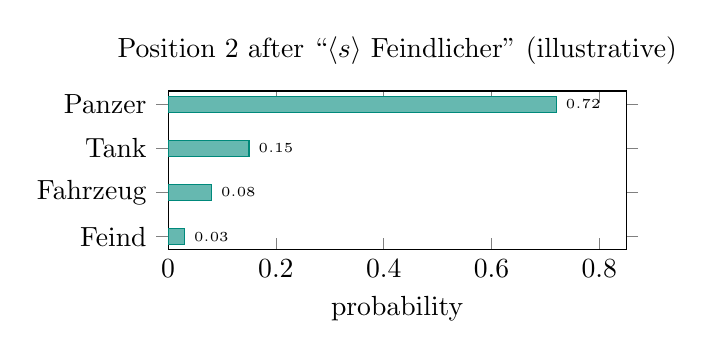
\begin{tikzpicture}
\begin{axis}[width=7.4cm,height=3.6cm,xbar,bar width=0.2cm,xmin=0,xmax=0.85,ytick=data,yticklabels={Panzer,Tank,Fahrzeug,Feind},y dir=reverse,xlabel={probability},title={Position 2 after ``$\langle s\rangle$ Feindlicher'' (illustrative)},nodes near coords,nodes near coords style={font=\fontsize{5.5}{6.5}\selectfont,/pgf/number format/.cd,fixed,precision=2}]
\addplot[fill=AccentCol!60,draw=AccentCol] coordinates{(0.72,1)(0.15,2)(0.08,3)(0.03,4)};
\end{axis}
\end{tikzpicture}}
\begin{ibox}\scriptsize At inference the paper used \textbf{beam search} (beam size 4) rather than always taking the single most likely word.\end{ibox}
\end{columns}
\end{frame}

\begin{frame}{Three Uses of Attention in One Model}
\centering\footnotesize\renewcommand{\arraystretch}{1.4}
\begin{tabularx}{\textwidth}{>{\bfseries}p{3.3cm} X X X}
\toprule
& \textbf{Encoder self-attention} \cn{3} & \textbf{Decoder masked self-attention} \cn{4} & \textbf{Encoder--decoder attention} \cn{5}\\\midrule
Queries from & source words & target words so far & target words so far\\
Keys \& values from & source words & target words so far & encoder output (source)\\
Mask & none & causal ($-\infty$ above diagonal) & none\\
Score matrix (example) & $3\times3$ & $5\times5$, lower triangle & $5\times3$\\
Question it answers & ``how do the English words relate?'' & ``what have I written so far?'' & ``which English words do I translate next?''\\\bottomrule
\end{tabularx}
\vspace{6pt}
\begin{rbox}\scriptsize The \emph{same} scaled dot-product attention formula is used in all three places; only the sources of $Q$, $K$, $V$ and the mask differ.\end{rbox}
\end{frame}

\begin{frame}{The Paper's Settings and Results}
\begin{columns}[T]
\column{0.52\textwidth}
\centering\scriptsize\renewcommand{\arraystretch}{1.22}
\begin{tabular}{lrr}
\toprule
&\textbf{Base}&\textbf{Big}\\\midrule
layers $N$ (each tower)&6&6\\
$d_{\text{model}}$&512&1024\\
$d_{ff}$ (FFN hidden)&2048&4096\\
heads $h$&8&16\\
$d_k=d_v$&64&64\\
dropout $P_{\text{drop}}$&0.1&0.3\\
parameters&65 M&213 M\\
training (8 NVIDIA P100 GPUs)&12 h&3.5 days\\\midrule
BLEU, WMT 2014 English--German&27.3&\textbf{28.4}\\
BLEU, WMT 2014 English--French&38.1&\textbf{41.8}\\\bottomrule
\end{tabular}
\column{0.45\textwidth}
\begin{cbox}{Training recipe}\scriptsize
\begin{tl}
\item Adam optimiser, $\beta_1=0.9$, $\beta_2=0.98$
\item learning rate warms up for 4\,000 steps, then decays: $\text{lr}=d_{\text{model}}^{-0.5}\min(\text{step}^{-0.5},\ \text{step}\cdot4000^{-1.5})$
\item dropout and label smoothing for regularisation
\item English--German: $\approx$4.5 M sentence pairs, $\approx$37\,000-token shared vocabulary
\end{tl}
\end{cbox}
\begin{rbox}\scriptsize The big model beat the previous best English--German results, including ensembles, by more than 2 BLEU --- at a fraction of their training cost.\end{rbox}
\begin{ibox}\scriptsize English--French big model: dropout 0.1. Figures from the paper's Tables 2 and 3.\end{ibox}
\end{columns}
\end{frame}

\begin{frame}{Three Families of Transformer Models}
\centering\footnotesize\renewcommand{\arraystretch}{1.35}
\begin{tabularx}{\textwidth}{>{\bfseries}p{2.3cm} X X X}
\toprule
& \textbf{Encoder-only} & \textbf{Decoder-only} & \textbf{Encoder--decoder}\\
\midrule
Which half of Fig.~1 & left tower & right tower without \cn{5} & both towers (the original)\\
Examples & BERT, RoBERTa & GPT series, Claude, Llama & original Transformer, T5, BART\\
Attention & bidirectional, no mask & causal mask & encoder bidirectional; decoder causal + cross\\
Trained to & fill in masked words & predict the next token & map input text to output text\\
Defence example & tag units, places and equipment in intercepts & draft a SITREP from field notes & translate captured documents\\
\bottomrule
\end{tabularx}
\vspace{4pt}
\begin{columns}[T]
\column{0.48\textwidth}
\begin{ibox}\scriptsize Same building block throughout; the families differ only in the mask, the wiring and the training objective.\end{ibox}
\column{0.48\textwidth}
\begin{cbox}{Scale}\scriptsize BERT-base $\approx$110 M parameters (2018); GPT-2 1.5 B (2019); GPT-3 175 B (2020).\end{cbox}
\end{columns}
\end{frame}

%====================================================================
\sect{9. Generation \& Training}
\begin{frame}{How a GPT-Style Model Writes: Next-Token Prediction}
\begin{columns}[T]
\column{0.54\textwidth}
\figc{2.0cm}{%
\begin{tikzpicture}[node distance=0.2cm]
\node[tok] (a) {The}; \node[tok,right=of a] (b) {convoy}; \node[tok,right=of b] (c) {crossed}; \node[tok,right=of c] (d) {the}; \node[tok,right=of d,draw=AccentCol,fill=AccentCol!20] (e) {?};
\node[ndC,above=0.5cm of c,minimum width=5.5cm] (m) {decoder blocks (causal attention)};
\foreach \n in {a,b,c,d}{\draw[arr] (\n.north)--(\n.north|-m.south);}
\draw[arrA] (m.east)-|(e.north);
\end{tikzpicture}}
\figc{3.2cm}{%
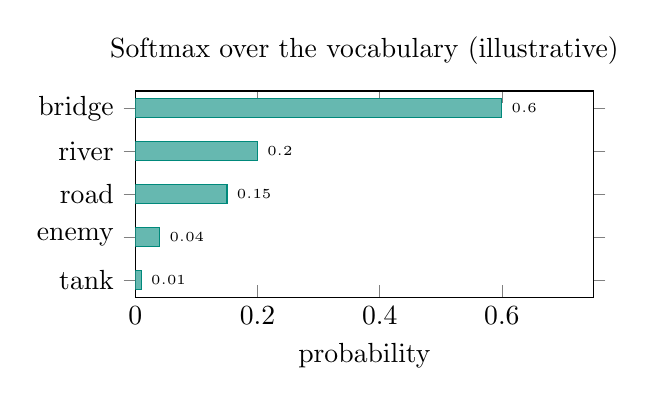
\begin{tikzpicture}
\begin{axis}[width=7.4cm,height=4.2cm,xbar,bar width=0.24cm,xmin=0,xmax=0.75,ytick=data,yticklabels={bridge,river,road,enemy,tank},y dir=reverse,xlabel={probability},title={Softmax over the vocabulary (illustrative)},nodes near coords,nodes near coords style={font=\fontsize{5.5}{6.5}\selectfont,/pgf/number format/.cd,fixed,precision=2}]
\addplot[fill=AccentCol!60,draw=AccentCol] coordinates{(0.60,1)(0.20,2)(0.15,3)(0.04,4)(0.01,5)};
\end{axis}
\end{tikzpicture}}
\column{0.43\textwidth}
\begin{cbox}{The loop}
\begin{te}
\item Run the prompt through all blocks
\item The last position's vector $\times$ an output matrix gives a score (logit) for every token in the vocabulary
\item Softmax $\to$ probabilities; pick or sample a token (``bridge'')
\item Append it and repeat
\end{te}
\end{cbox}
\begin{ibox}\scriptsize\textbf{Temperature} $\tau$: softmax of logits$/\tau$. Low $\tau$ $\to$ predictable; high $\tau$ $\to$ varied. Logits here: $(3.2,2.1,1.8,0.4,-0.5)$.\end{ibox}
\end{columns}
\end{frame}

\begin{frame}{How Transformers Are Trained}
\begin{columns}[T]
\column{0.50\textwidth}
\begin{cbox}{Pre-training: predict the next token}
For every position $t$ in billions of sentences, the loss is the cross-entropy of the true next token:
\[L=-\frac1T\sum_{t=1}^{T}\ln P_\theta(w_{t+1}\mid w_1,\dots,w_t)\]
In the example, if the true word is ``bridge'': $L=-\ln0.60=0.51$.
\end{cbox}
\begin{rbox}\scriptsize The causal mask lets one forward pass produce a prediction --- and a loss term --- at \emph{every} position simultaneously. That parallelism is why transformers train so efficiently.\end{rbox}
\column{0.47\textwidth}
\begin{cbox}[ISSAnavy]{Then backpropagation, as before}
The gradient flows back through softmax, $W^O$, every head's $W^Q,W^K,W^V$, the FFNs and the embedding table --- the same chain rule as Lecture~6 (backpropagation by hand), just with more layers.
\end{cbox}
\begin{cbox}{After pre-training}
\begin{tl}
\item \textbf{Fine-tuning} on a smaller, task-specific dataset
\item \textbf{Instruction tuning} and \textbf{human-feedback} training to follow requests helpfully and safely
\item Or no training at all: give examples in the prompt (\emph{in-context learning})
\end{tl}
\end{cbox}
\end{columns}
\end{frame}

%====================================================================
\sect{10. Defence Applications}
\begin{frame}{Transformers in Defence and Wargaming}
\begin{columns}[T]
\column{0.49\textwidth}
\begin{cbox}{Text and intelligence}\scriptsize Summarising reports, extracting entities (units, locations, equipment) from intercepts, translating captured documents, searching archives by meaning rather than keyword.\end{cbox}
\begin{cbox}{Imagery (Vision Transformer)}\scriptsize Cut a SAR or EO image into $16\times16$ patches; each patch is a ``token'' with its own positional encoding. Attention links distant parts of a scene --- e.g.\ vehicles and the road network they use.\end{cbox}
\begin{cbox}{Sensor fusion and tracks}\scriptsize Each radar track or sensor report becomes a token; attention learns which tracks relate (formation flying, escort--target pairs).\end{cbox}
\column{0.48\textwidth}
\begin{cbox}{Wargaming and decision support}\scriptsize Transformer policies over sets of units (any number of tokens), analysis of game logs to find decisive moments, natural-language interfaces to simulations.\end{cbox}
\begin{wbox}\scriptsize\textbf{Limits to brief commanders on}
\begin{tl}
\item \textbf{Hallucination}: fluent, confident, wrong statements
\item \textbf{Prompt injection}: hostile text inside a document can redirect the model
\item \textbf{Distribution shift}: trained on open text, deployed on jargon and new theatres
\item \textbf{Cost}: attention is $O(n^2)$ in sequence length
\end{tl}\end{wbox}
\end{columns}
\end{frame}

\begin{frame}{Common Misconceptions}
\begin{columns}[T]
\column{0.49\textwidth}
\begin{wbox}\textbf{``Attention = understanding.''}\ \scriptsize Attention is a weighted average learned to reduce prediction error. Whether that amounts to understanding is a separate question.\end{wbox}
\begin{wbox}\textbf{``Q, K, V are three different inputs.''}\ \scriptsize In self-attention they are three \emph{projections of the same} input $X$.\end{wbox}
\begin{wbox}\textbf{``Positional encoding is concatenated.''}\ \scriptsize It is \emph{added}, element by element, to the embedding.\end{wbox}
\begin{wbox}\textbf{``Embedding dimensions have names.''}\ \scriptsize Only in our toy; real dimensions are unlabelled and meaning is spread across them.\end{wbox}
\column{0.49\textwidth}
\begin{wbox}\textbf{``The model reads left to right.''}\ \scriptsize Only decoders are causal. Encoders see the whole sequence at once.\end{wbox}
\begin{wbox}\textbf{``Softmax picks the best word.''}\ \scriptsize It produces a full distribution; the decoding strategy (greedy, beam search, sampling) picks.\end{wbox}
\begin{wbox}\textbf{``Bigger context is free.''}\ \scriptsize Doubling the sequence length quadruples the attention score matrix: $n\times n$.\end{wbox}
\begin{ibox}\scriptsize\textbf{Self-check:} if you can reproduce the worked example and label every block of Figure~1, you understand the core of every transformer.\end{ibox}
\end{columns}
\end{frame}

\sect{11. Summary}
\begin{frame}{Summary and Quick Check}
\begin{columns}[T]
\column{0.55\textwidth}
\begin{fbx}{Input}$h_0=\sqrt{d_{\text{model}}}\,\text{Embed}(\text{tokens})+PE$\end{fbx}
\begin{fbx}{Positional encoding}$PE_{(pos,2i)}=\sin(pos/10000^{2i/d}),\ PE_{(pos,2i+1)}=\cos(\cdot)$\end{fbx}
\begin{fbx}{Attention}$\text{softmax}\bigl(QK^{\mathsf T}/\sqrt{d_k}\,[+M]\bigr)\,V$, \ $Q=XW^Q,\ K=XW^K,\ V=XW^V$\end{fbx}
\begin{fbx}{Multi-head}$\text{Concat}(\text{head}_1,\dots,\text{head}_h)\,W^O$\end{fbx}
\begin{fbx}{Each sub-layer}$\text{LayerNorm}(x+\text{Sublayer}(x))$\end{fbx}
\column{0.42\textwidth}
\begin{cbox}{Quick check}
\begin{te}
\item Using the toy table, compute \emph{lion}\,$-$\,\emph{man}\,$+$\,\emph{woman} (lion $=(0.85,0,0.90,0.30)$). Which word is nearest?
\item Compute $p_3$ for $d_{\text{model}}=4$.
\item In head 1, which word does ``tank'' attend to most, and with what weight?
\item Why must the multi-head output have the same width as $X$?
\item In Figure~1, where do the keys and values of block \cn{5} come from, and why is no mask needed there?
\end{te}
\end{cbox}
\end{columns}
\end{frame}


\begin{frame}{Looking Ahead --- Lecture 10: Reinforcement Learning Part 1 --- Q-Learning \& MDPs}
\begin{columns}[T]
\column{0.50\textwidth}
\subhead{From passive learning to active decision-making}
\begin{tl}\item RL vs supervised / unsupervised\item MDP: $S$, $A$, $P(s'|s,a)$, $R(s,a,s')$, $\gamma$\item Bellman optimality: $V^*(s)$, $Q^*(s,a)$ derived from scratch\item Q-learning: TD update, $\varepsilon$-greedy, convergence\item DQN: a neural network --- trained by backpropagation (L6) --- replaces the Q-table; experience replay; target network\end{tl}
\begin{ibox}\scriptsize\textbf{Assignment 9:} sinusoidal positional encoding + scaled dot-product attention by hand + multi-head shapes and parameter counts + masking and cost + BERT vs GPT for a defence task; bonus: Add \& Norm by hand.\end{ibox}
\column{0.46\textwidth}
\begin{cbox}{Preview: wargame tactical agent}\scriptsize $20\times20$ hex JANUS map; state space $\sim10^{28}$ (no Q-table can hold it); actions \{move N/S/E/W, attack, defend, resupply\}; reward $+10$ objective, $+5$ kill, $-8$ unit lost.\end{cbox}
\figc{2.3cm}{\bars{100}{1.6}{2.0}{Tabular Q (10$\times$10) vs random/91/ISSAgrn,DQN (20$\times$20) vs novice human/81/ISSAblue,DQN vs minimax AI/54/ISSAamb}}
\sm{DQN: 3 layers $\times$ 512 units; 100K-transition replay buffer; target update every 1,000 steps; 100K episodes, 48 GPU-hours.}
\end{columns}
\end{frame}
\end{document}
